\begin{table}[htbp]
\centering
\small
\caption{Index of per-analysis count-support and selection summaries. Every one of the 158 analysis runs appears on exactly one page.}
\label{tab:why-index}
\begin{tabular}{llrr}
\toprule
Scheme & Family & Runs & Figures \\
\midrule
Parameter resampling & PDZ & 14 & \ref{fig:why-parameter_posterior-pdz-1}--\ref{fig:why-parameter_posterior-pdz-5} \\
Parameter resampling & TrpB & 28 & \ref{fig:why-parameter_posterior-trpb-1}--\ref{fig:why-parameter_posterior-trpb-10} \\
Parameter resampling & NucB & 7 & \ref{fig:why-parameter_posterior-nuc-1}--\ref{fig:why-parameter_posterior-nuc-3} \\
Optimized-fit count resampling & PDZ & 19 & \ref{fig:why-mle_predictive-pdz-1}--\ref{fig:why-mle_predictive-pdz-7} \\
Optimized-fit count resampling & TrpB & 34 & \ref{fig:why-mle_predictive-trpb-1}--\ref{fig:why-mle_predictive-trpb-12} \\
Optimized-fit count resampling & NucB & 7 & \ref{fig:why-mle_predictive-nuc-1}--\ref{fig:why-mle_predictive-nuc-3} \\
Posterior count resampling & PDZ & 14 & \ref{fig:why-posterior_predictive-pdz-1}--\ref{fig:why-posterior_predictive-pdz-5} \\
Posterior count resampling & TrpB & 28 & \ref{fig:why-posterior_predictive-trpb-1}--\ref{fig:why-posterior_predictive-trpb-10} \\
Posterior count resampling & NucB & 7 & \ref{fig:why-posterior_predictive-nuc-1}--\ref{fig:why-posterior_predictive-nuc-3} \\
\bottomrule
\end{tabular}
\end{table}
\clearpage

\begin{figure}[p]
\centering
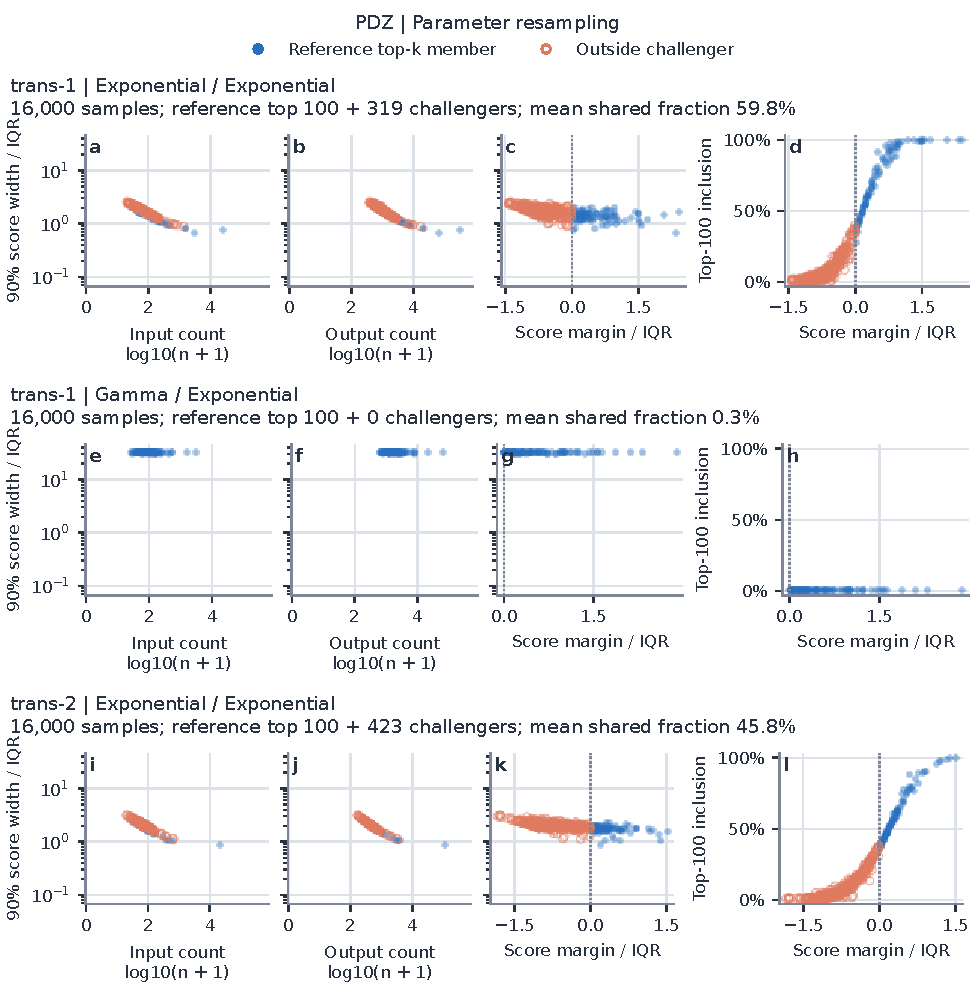
\includegraphics[width=\linewidth]{summary_why_parameter_posterior_pdz_01.pdf}
\caption{PDZ decision-cohort summaries: parameter resampling. Rows, top to bottom: pdz-trans-1, Exponential--Exponential; pdz-trans-1, Gamma--Exponential; pdz-trans-2, Exponential--Exponential. Columns show normalized central 90\% score width versus input count, output count, and median-score margin from the top-100 cutoff; then top-100 inclusion versus that margin. Widths and margins use the run's top-1,000 median-score interquartile range (IQR). Blue filled points are reference top-100 members; orange open points are outside candidates with inclusion probability at least 0.01. Count and score-width limits are shared within family and scheme; margin limits are shared within a row. Dotted lines mark the cutoff. No regression lines are fitted.}
\label{fig:why-parameter_posterior-pdz-1}
\end{figure}
\clearpage

\begin{figure}[p]
\centering
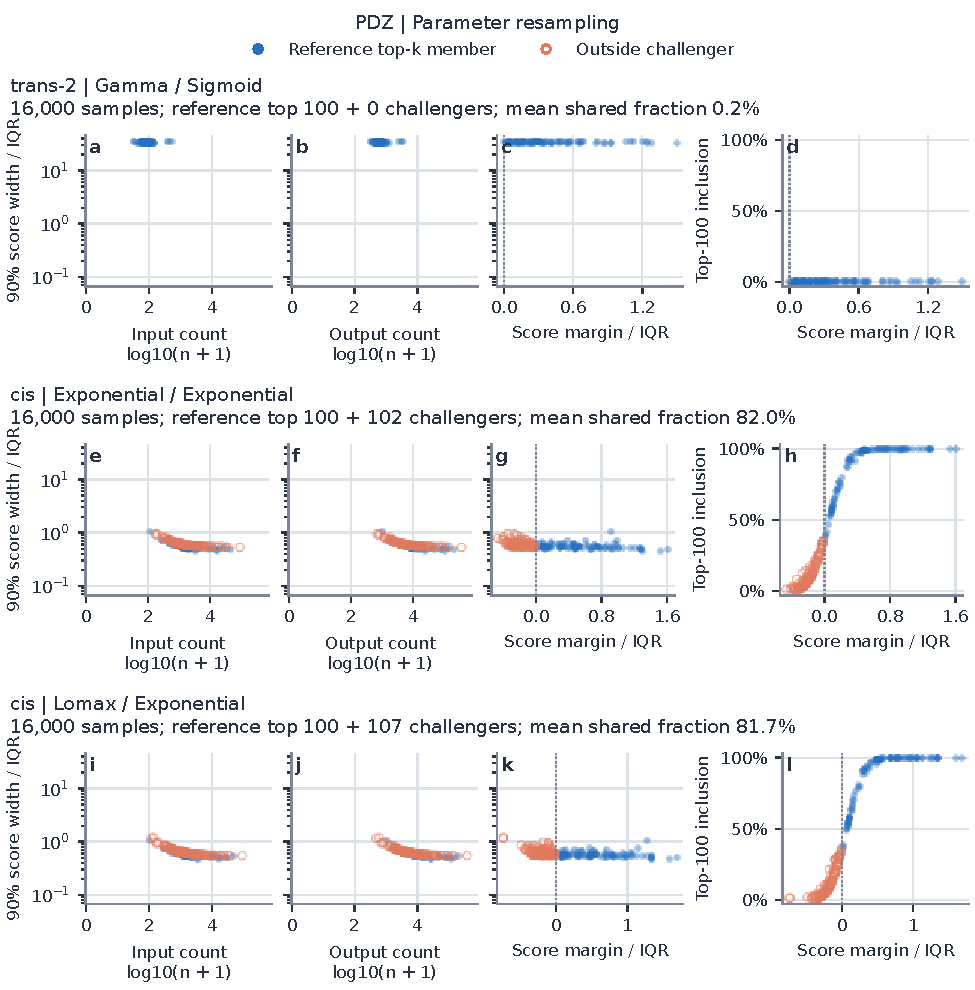
\includegraphics[width=\linewidth]{summary_why_parameter_posterior_pdz_02.pdf}
\caption{PDZ decision-cohort summaries: parameter resampling. Rows, top to bottom: pdz-trans-2, Gamma--Sigmoid; pdz-cis, Exponential--Exponential; pdz-cis, Lomax--Exponential. Columns show normalized central 90\% score width versus input count, output count, and median-score margin from the top-100 cutoff; then top-100 inclusion versus that margin. Widths and margins use the run's top-1,000 median-score interquartile range (IQR). Blue filled points are reference top-100 members; orange open points are outside candidates with inclusion probability at least 0.01. Count and score-width limits are shared within family and scheme; margin limits are shared within a row. Dotted lines mark the cutoff. No regression lines are fitted.}
\label{fig:why-parameter_posterior-pdz-2}
\end{figure}
\clearpage

\begin{figure}[p]
\centering
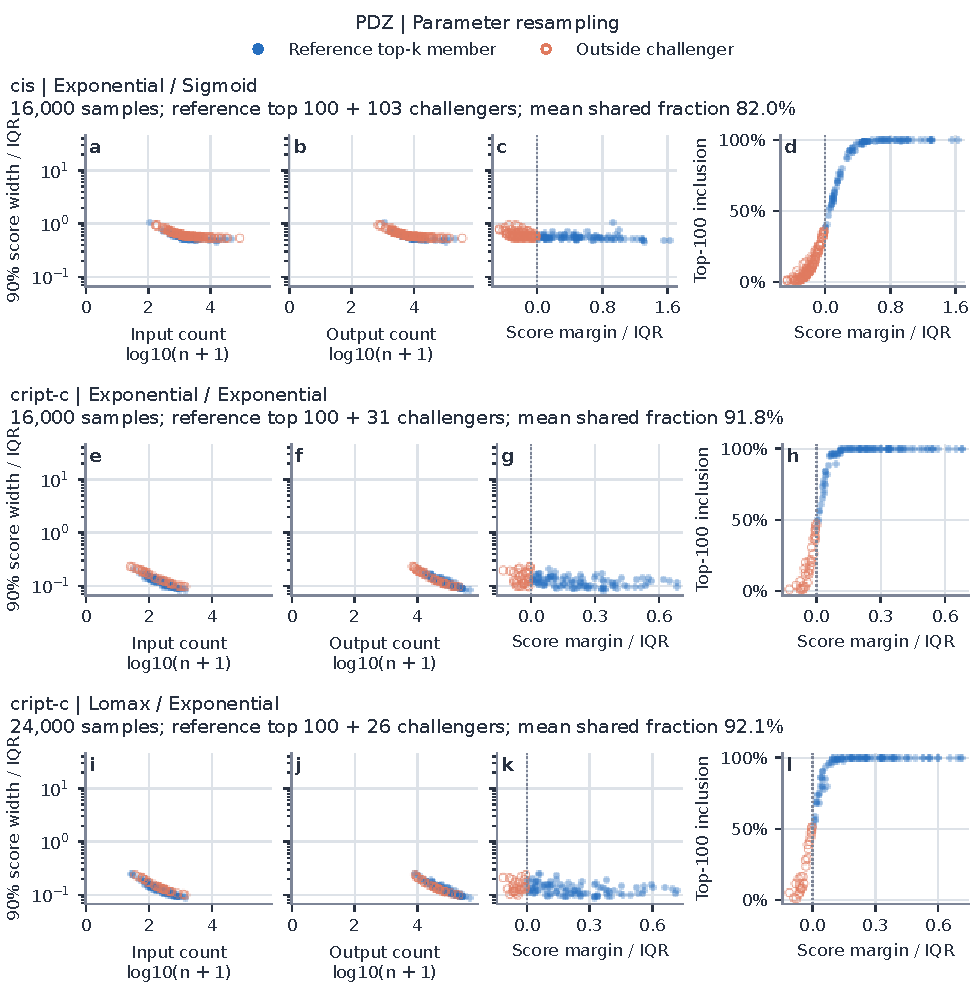
\includegraphics[width=\linewidth]{summary_why_parameter_posterior_pdz_03.pdf}
\caption{PDZ decision-cohort summaries: parameter resampling. Rows, top to bottom: pdz-cis, Exponential--Sigmoid; pdz-cript-c, Exponential--Exponential; pdz-cript-c, Lomax--Exponential. Columns show normalized central 90\% score width versus input count, output count, and median-score margin from the top-100 cutoff; then top-100 inclusion versus that margin. Widths and margins use the run's top-1,000 median-score interquartile range (IQR). Blue filled points are reference top-100 members; orange open points are outside candidates with inclusion probability at least 0.01. Count and score-width limits are shared within family and scheme; margin limits are shared within a row. Dotted lines mark the cutoff. No regression lines are fitted.}
\label{fig:why-parameter_posterior-pdz-3}
\end{figure}
\clearpage

\begin{figure}[p]
\centering
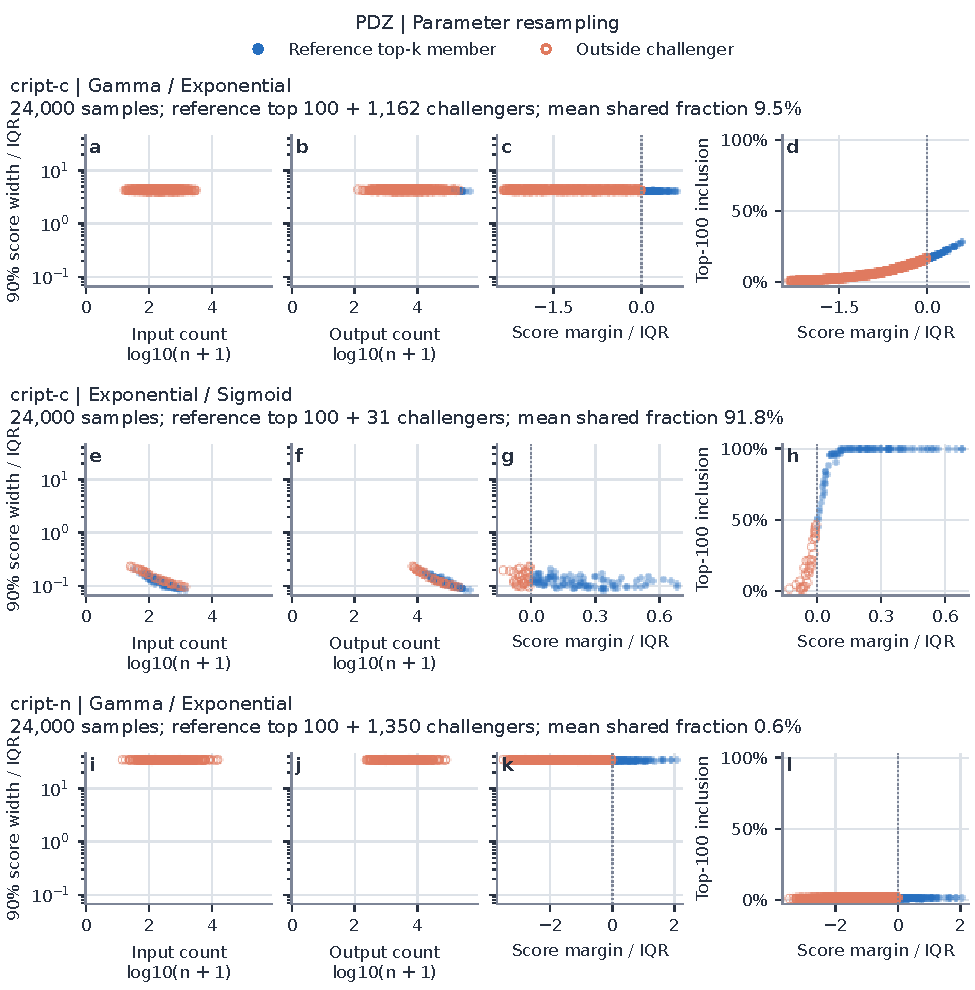
\includegraphics[width=\linewidth]{summary_why_parameter_posterior_pdz_04.pdf}
\caption{PDZ decision-cohort summaries: parameter resampling. Rows, top to bottom: pdz-cript-c, Gamma--Exponential; pdz-cript-c, Exponential--Sigmoid; pdz-cript-n, Gamma--Exponential. Columns show normalized central 90\% score width versus input count, output count, and median-score margin from the top-100 cutoff; then top-100 inclusion versus that margin. Widths and margins use the run's top-1,000 median-score interquartile range (IQR). Blue filled points are reference top-100 members; orange open points are outside candidates with inclusion probability at least 0.01. Count and score-width limits are shared within family and scheme; margin limits are shared within a row. Dotted lines mark the cutoff. No regression lines are fitted.}
\label{fig:why-parameter_posterior-pdz-4}
\end{figure}
\clearpage

\begin{figure}[p]
\centering
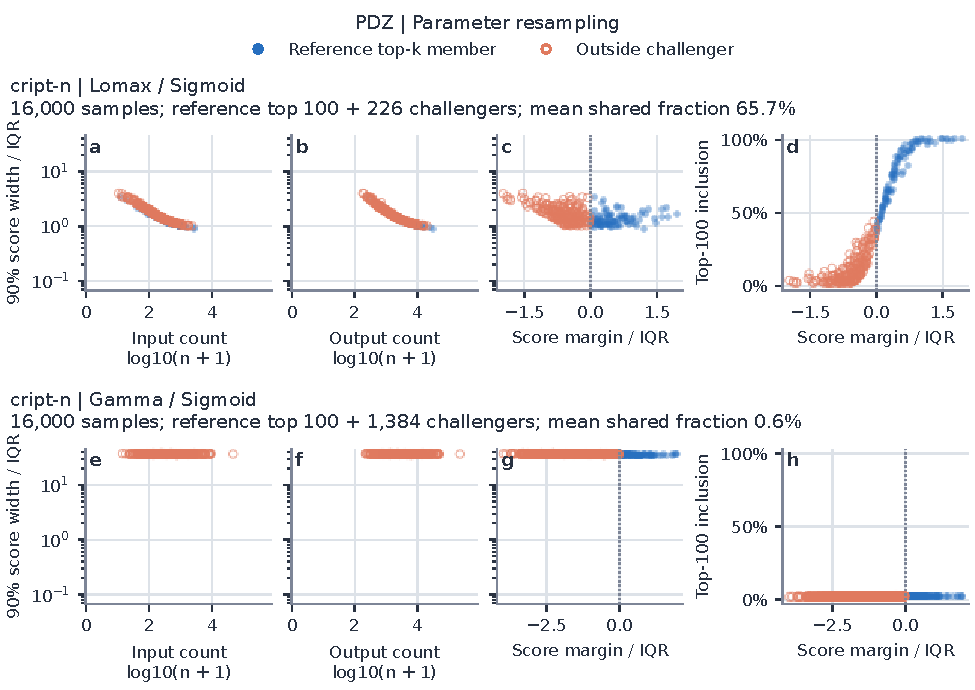
\includegraphics[width=\linewidth]{summary_why_parameter_posterior_pdz_05.pdf}
\caption{PDZ decision-cohort summaries: parameter resampling. Rows, top to bottom: pdz-cript-n, Lomax--Sigmoid; pdz-cript-n, Gamma--Sigmoid. Columns show normalized central 90\% score width versus input count, output count, and median-score margin from the top-100 cutoff; then top-100 inclusion versus that margin. Widths and margins use the run's top-1,000 median-score interquartile range (IQR). Blue filled points are reference top-100 members; orange open points are outside candidates with inclusion probability at least 0.01. Count and score-width limits are shared within family and scheme; margin limits are shared within a row. Dotted lines mark the cutoff. No regression lines are fitted.}
\label{fig:why-parameter_posterior-pdz-5}
\end{figure}
\clearpage

\begin{figure}[p]
\centering
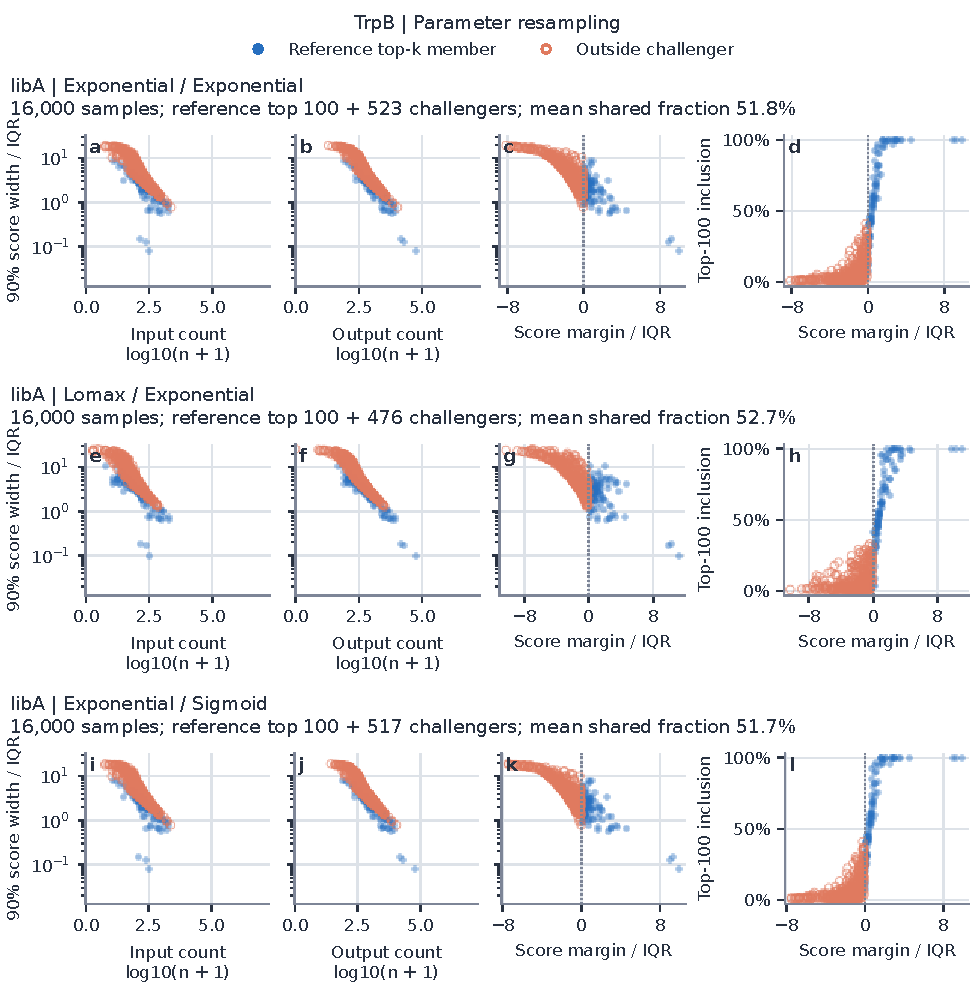
\includegraphics[width=\linewidth]{summary_why_parameter_posterior_trpb_01.pdf}
\caption{TrpB decision-cohort summaries: parameter resampling. Rows, top to bottom: trpb-libA, Exponential--Exponential; trpb-libA, Lomax--Exponential; trpb-libA, Exponential--Sigmoid. Columns show normalized central 90\% score width versus input count, output count, and median-score margin from the top-100 cutoff; then top-100 inclusion versus that margin. Widths and margins use the run's top-1,000 median-score interquartile range (IQR). Blue filled points are reference top-100 members; orange open points are outside candidates with inclusion probability at least 0.01. Count and score-width limits are shared within family and scheme; margin limits are shared within a row. Dotted lines mark the cutoff. No regression lines are fitted.}
\label{fig:why-parameter_posterior-trpb-1}
\end{figure}
\clearpage

\begin{figure}[p]
\centering
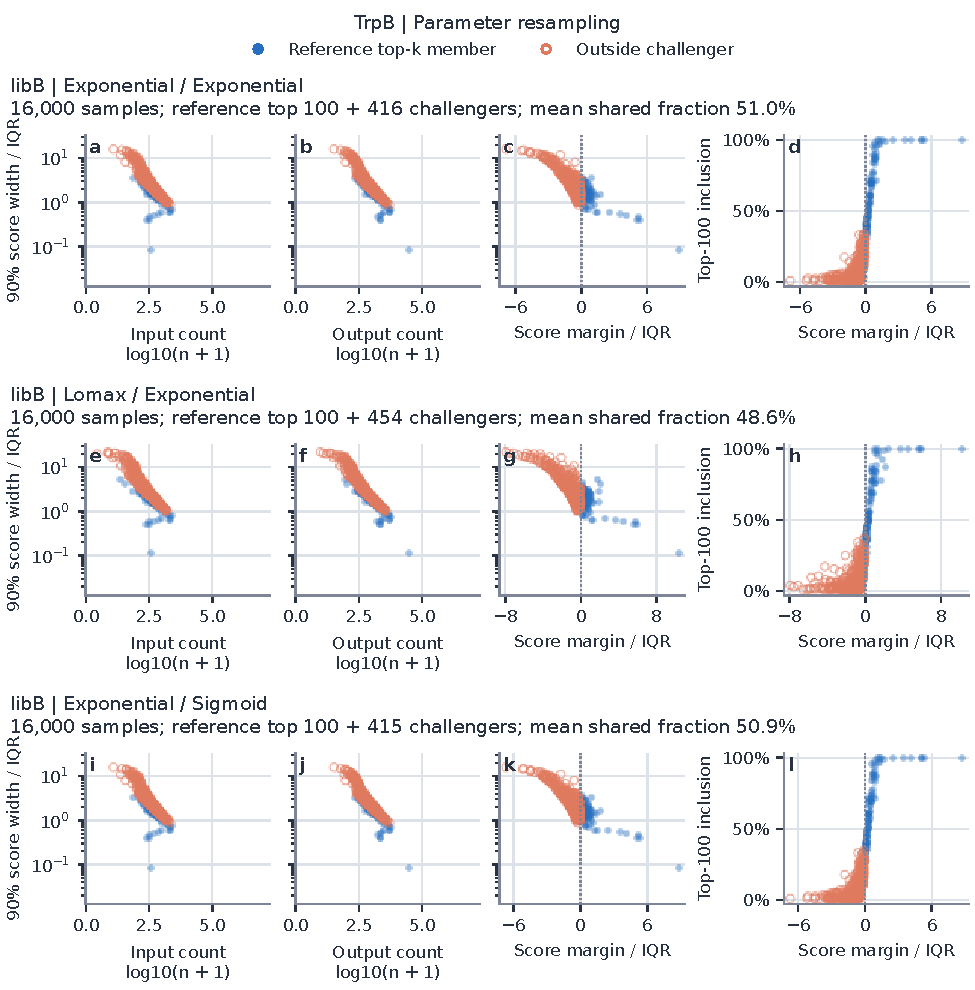
\includegraphics[width=\linewidth]{summary_why_parameter_posterior_trpb_02.pdf}
\caption{TrpB decision-cohort summaries: parameter resampling. Rows, top to bottom: trpb-libB, Exponential--Exponential; trpb-libB, Lomax--Exponential; trpb-libB, Exponential--Sigmoid. Columns show normalized central 90\% score width versus input count, output count, and median-score margin from the top-100 cutoff; then top-100 inclusion versus that margin. Widths and margins use the run's top-1,000 median-score interquartile range (IQR). Blue filled points are reference top-100 members; orange open points are outside candidates with inclusion probability at least 0.01. Count and score-width limits are shared within family and scheme; margin limits are shared within a row. Dotted lines mark the cutoff. No regression lines are fitted.}
\label{fig:why-parameter_posterior-trpb-2}
\end{figure}
\clearpage

\begin{figure}[p]
\centering
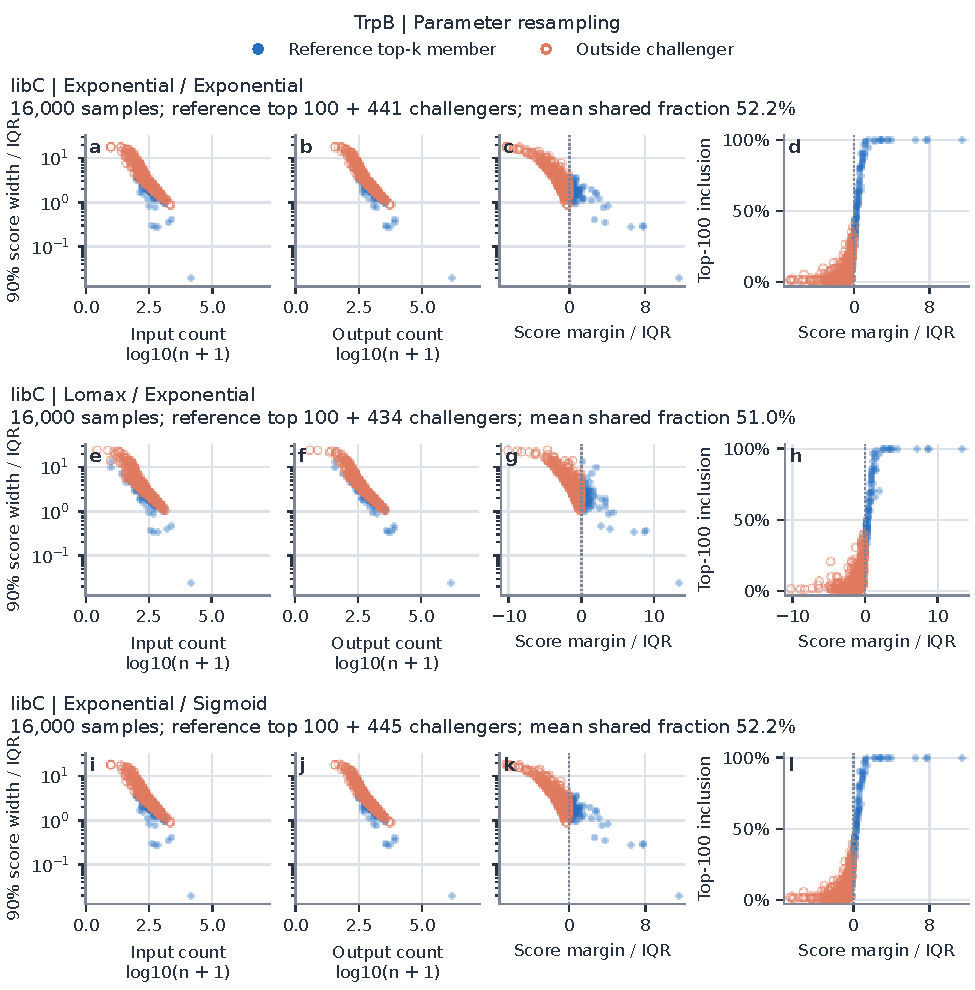
\includegraphics[width=\linewidth]{summary_why_parameter_posterior_trpb_03.pdf}
\caption{TrpB decision-cohort summaries: parameter resampling. Rows, top to bottom: trpb-libC, Exponential--Exponential; trpb-libC, Lomax--Exponential; trpb-libC, Exponential--Sigmoid. Columns show normalized central 90\% score width versus input count, output count, and median-score margin from the top-100 cutoff; then top-100 inclusion versus that margin. Widths and margins use the run's top-1,000 median-score interquartile range (IQR). Blue filled points are reference top-100 members; orange open points are outside candidates with inclusion probability at least 0.01. Count and score-width limits are shared within family and scheme; margin limits are shared within a row. Dotted lines mark the cutoff. No regression lines are fitted.}
\label{fig:why-parameter_posterior-trpb-3}
\end{figure}
\clearpage

\begin{figure}[p]
\centering
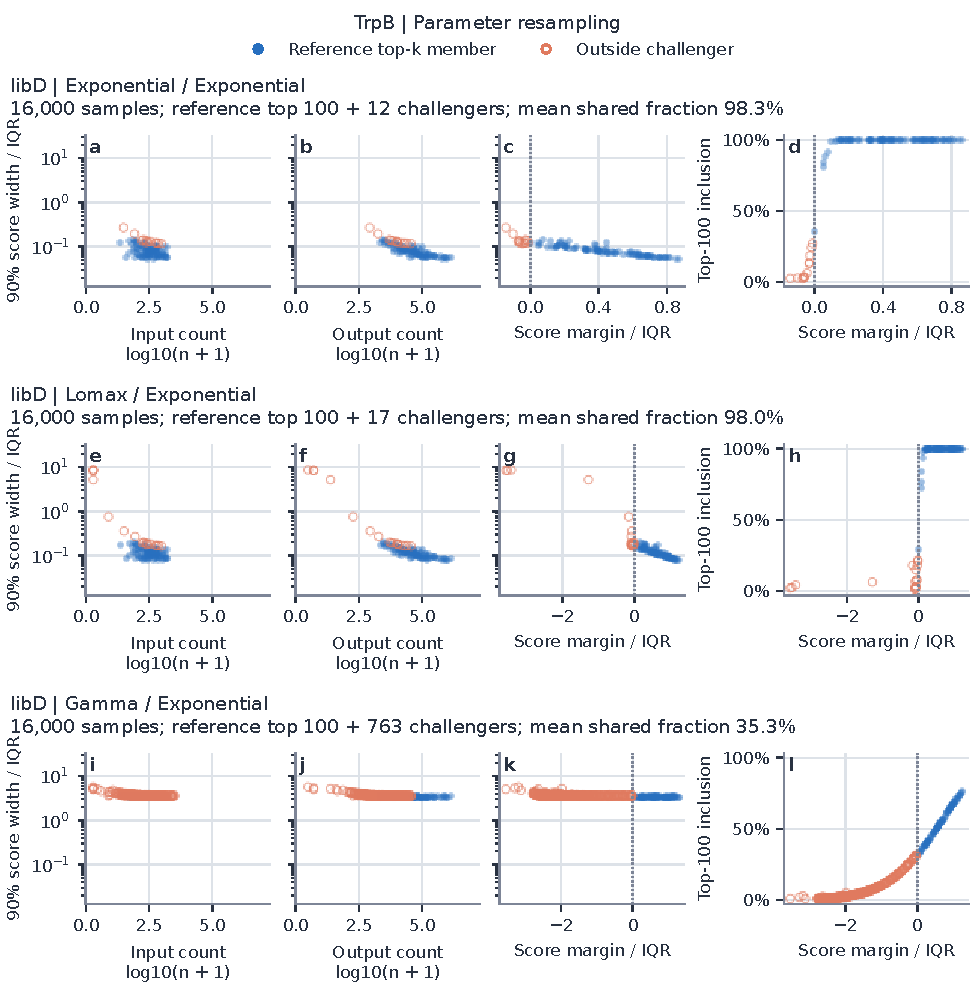
\includegraphics[width=\linewidth]{summary_why_parameter_posterior_trpb_04.pdf}
\caption{TrpB decision-cohort summaries: parameter resampling. Rows, top to bottom: trpb-libD, Exponential--Exponential; trpb-libD, Lomax--Exponential; trpb-libD, Gamma--Exponential. Columns show normalized central 90\% score width versus input count, output count, and median-score margin from the top-100 cutoff; then top-100 inclusion versus that margin. Widths and margins use the run's top-1,000 median-score interquartile range (IQR). Blue filled points are reference top-100 members; orange open points are outside candidates with inclusion probability at least 0.01. Count and score-width limits are shared within family and scheme; margin limits are shared within a row. Dotted lines mark the cutoff. No regression lines are fitted.}
\label{fig:why-parameter_posterior-trpb-4}
\end{figure}
\clearpage

\begin{figure}[p]
\centering
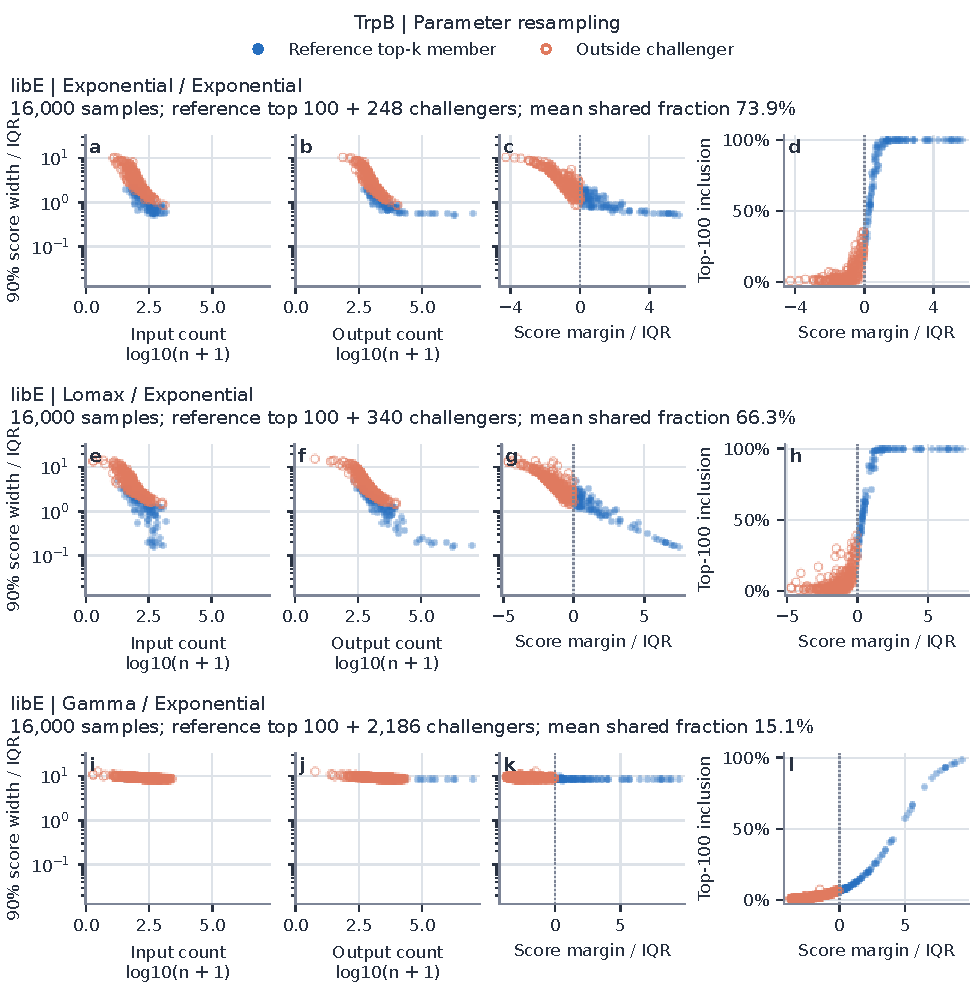
\includegraphics[width=\linewidth]{summary_why_parameter_posterior_trpb_05.pdf}
\caption{TrpB decision-cohort summaries: parameter resampling. Rows, top to bottom: trpb-libE, Exponential--Exponential; trpb-libE, Lomax--Exponential; trpb-libE, Gamma--Exponential. Columns show normalized central 90\% score width versus input count, output count, and median-score margin from the top-100 cutoff; then top-100 inclusion versus that margin. Widths and margins use the run's top-1,000 median-score interquartile range (IQR). Blue filled points are reference top-100 members; orange open points are outside candidates with inclusion probability at least 0.01. Count and score-width limits are shared within family and scheme; margin limits are shared within a row. Dotted lines mark the cutoff. No regression lines are fitted.}
\label{fig:why-parameter_posterior-trpb-5}
\end{figure}
\clearpage

\begin{figure}[p]
\centering
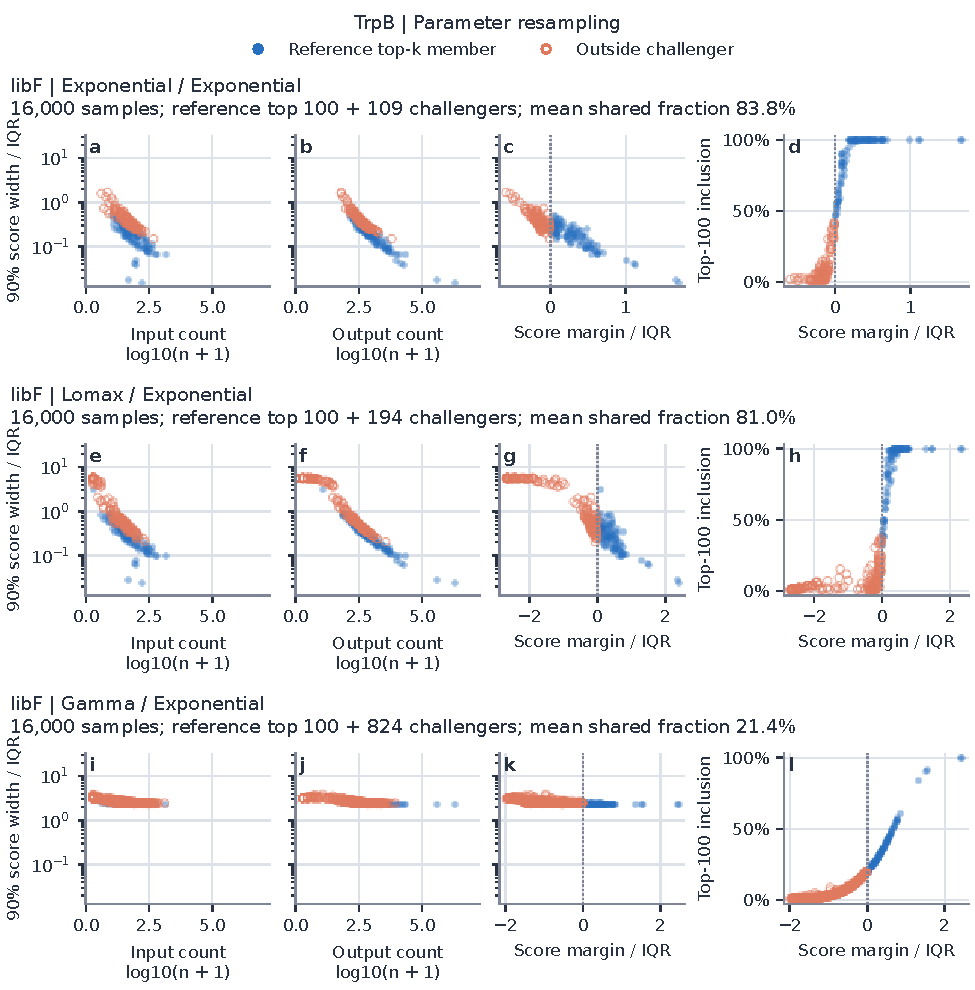
\includegraphics[width=\linewidth]{summary_why_parameter_posterior_trpb_06.pdf}
\caption{TrpB decision-cohort summaries: parameter resampling. Rows, top to bottom: trpb-libF, Exponential--Exponential; trpb-libF, Lomax--Exponential; trpb-libF, Gamma--Exponential. Columns show normalized central 90\% score width versus input count, output count, and median-score margin from the top-100 cutoff; then top-100 inclusion versus that margin. Widths and margins use the run's top-1,000 median-score interquartile range (IQR). Blue filled points are reference top-100 members; orange open points are outside candidates with inclusion probability at least 0.01. Count and score-width limits are shared within family and scheme; margin limits are shared within a row. Dotted lines mark the cutoff. No regression lines are fitted.}
\label{fig:why-parameter_posterior-trpb-6}
\end{figure}
\clearpage

\begin{figure}[p]
\centering
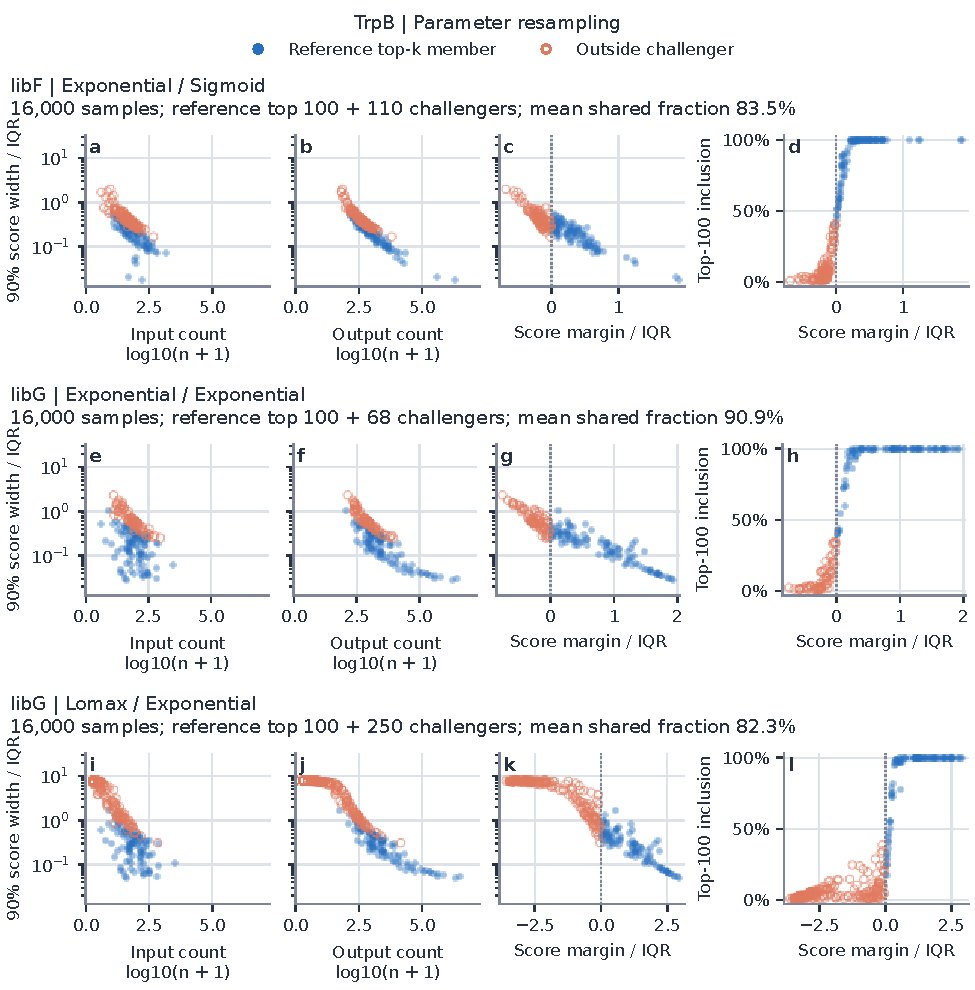
\includegraphics[width=\linewidth]{summary_why_parameter_posterior_trpb_07.pdf}
\caption{TrpB decision-cohort summaries: parameter resampling. Rows, top to bottom: trpb-libF, Exponential--Sigmoid; trpb-libG, Exponential--Exponential; trpb-libG, Lomax--Exponential. Columns show normalized central 90\% score width versus input count, output count, and median-score margin from the top-100 cutoff; then top-100 inclusion versus that margin. Widths and margins use the run's top-1,000 median-score interquartile range (IQR). Blue filled points are reference top-100 members; orange open points are outside candidates with inclusion probability at least 0.01. Count and score-width limits are shared within family and scheme; margin limits are shared within a row. Dotted lines mark the cutoff. No regression lines are fitted.}
\label{fig:why-parameter_posterior-trpb-7}
\end{figure}
\clearpage

\begin{figure}[p]
\centering
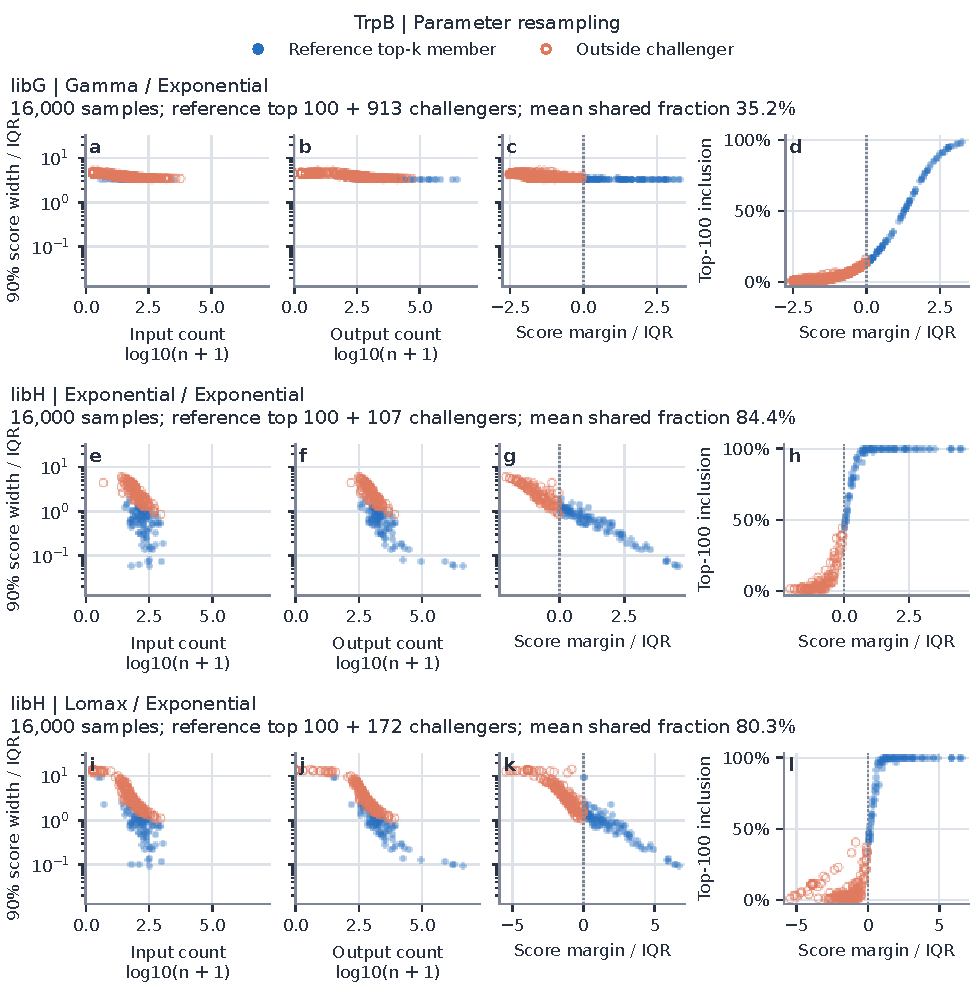
\includegraphics[width=\linewidth]{summary_why_parameter_posterior_trpb_08.pdf}
\caption{TrpB decision-cohort summaries: parameter resampling. Rows, top to bottom: trpb-libG, Gamma--Exponential; trpb-libH, Exponential--Exponential; trpb-libH, Lomax--Exponential. Columns show normalized central 90\% score width versus input count, output count, and median-score margin from the top-100 cutoff; then top-100 inclusion versus that margin. Widths and margins use the run's top-1,000 median-score interquartile range (IQR). Blue filled points are reference top-100 members; orange open points are outside candidates with inclusion probability at least 0.01. Count and score-width limits are shared within family and scheme; margin limits are shared within a row. Dotted lines mark the cutoff. No regression lines are fitted.}
\label{fig:why-parameter_posterior-trpb-8}
\end{figure}
\clearpage

\begin{figure}[p]
\centering
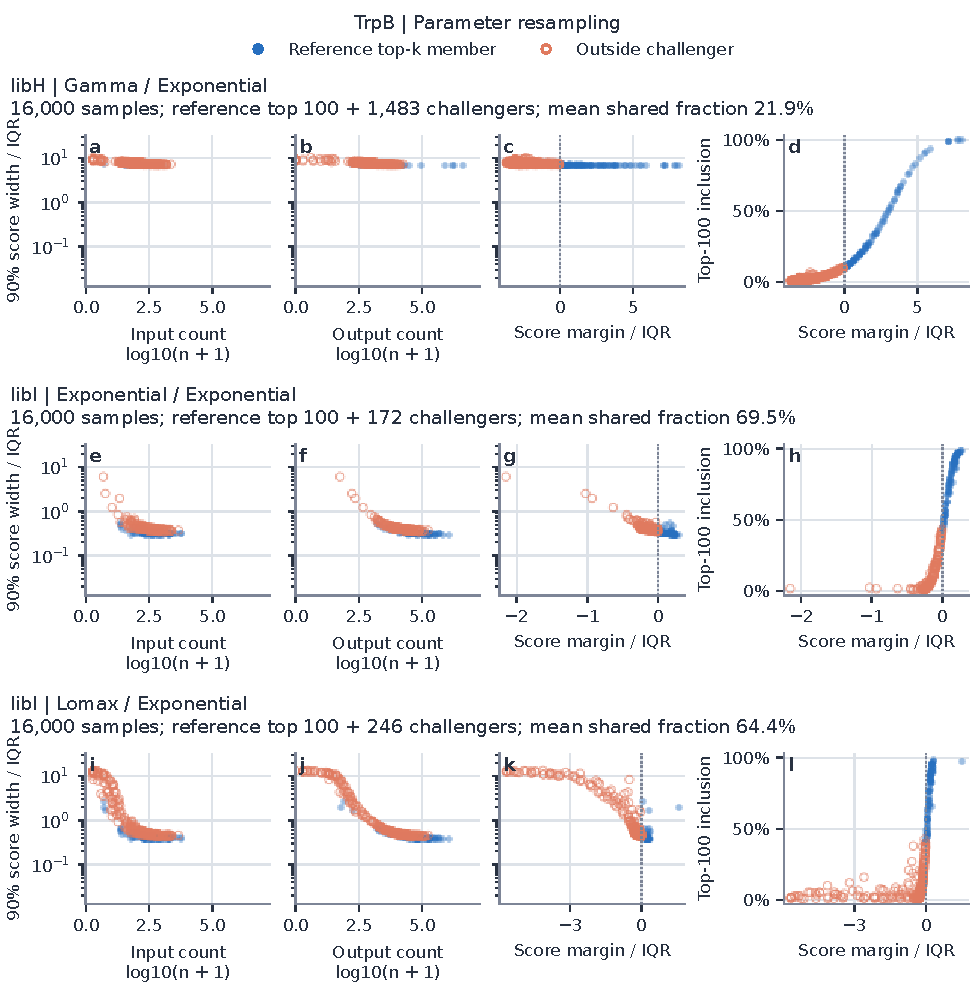
\includegraphics[width=\linewidth]{summary_why_parameter_posterior_trpb_09.pdf}
\caption{TrpB decision-cohort summaries: parameter resampling. Rows, top to bottom: trpb-libH, Gamma--Exponential; trpb-libI, Exponential--Exponential; trpb-libI, Lomax--Exponential. Columns show normalized central 90\% score width versus input count, output count, and median-score margin from the top-100 cutoff; then top-100 inclusion versus that margin. Widths and margins use the run's top-1,000 median-score interquartile range (IQR). Blue filled points are reference top-100 members; orange open points are outside candidates with inclusion probability at least 0.01. Count and score-width limits are shared within family and scheme; margin limits are shared within a row. Dotted lines mark the cutoff. No regression lines are fitted.}
\label{fig:why-parameter_posterior-trpb-9}
\end{figure}
\clearpage

\begin{figure}[p]
\centering
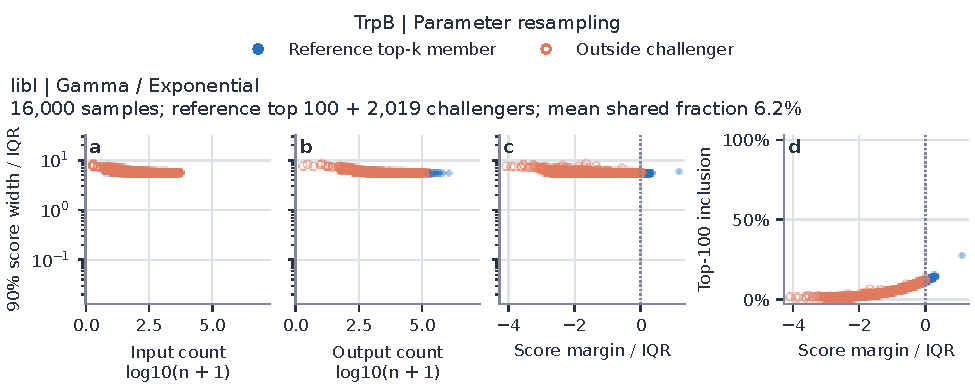
\includegraphics[width=\linewidth]{summary_why_parameter_posterior_trpb_10.pdf}
\caption{TrpB decision-cohort summaries: parameter resampling. Rows, top to bottom: trpb-libI, Gamma--Exponential. Columns show normalized central 90\% score width versus input count, output count, and median-score margin from the top-100 cutoff; then top-100 inclusion versus that margin. Widths and margins use the run's top-1,000 median-score interquartile range (IQR). Blue filled points are reference top-100 members; orange open points are outside candidates with inclusion probability at least 0.01. Count and score-width limits are shared within family and scheme; margin limits are shared within a row. Dotted lines mark the cutoff. No regression lines are fitted.}
\label{fig:why-parameter_posterior-trpb-10}
\end{figure}
\clearpage

\begin{figure}[p]
\centering
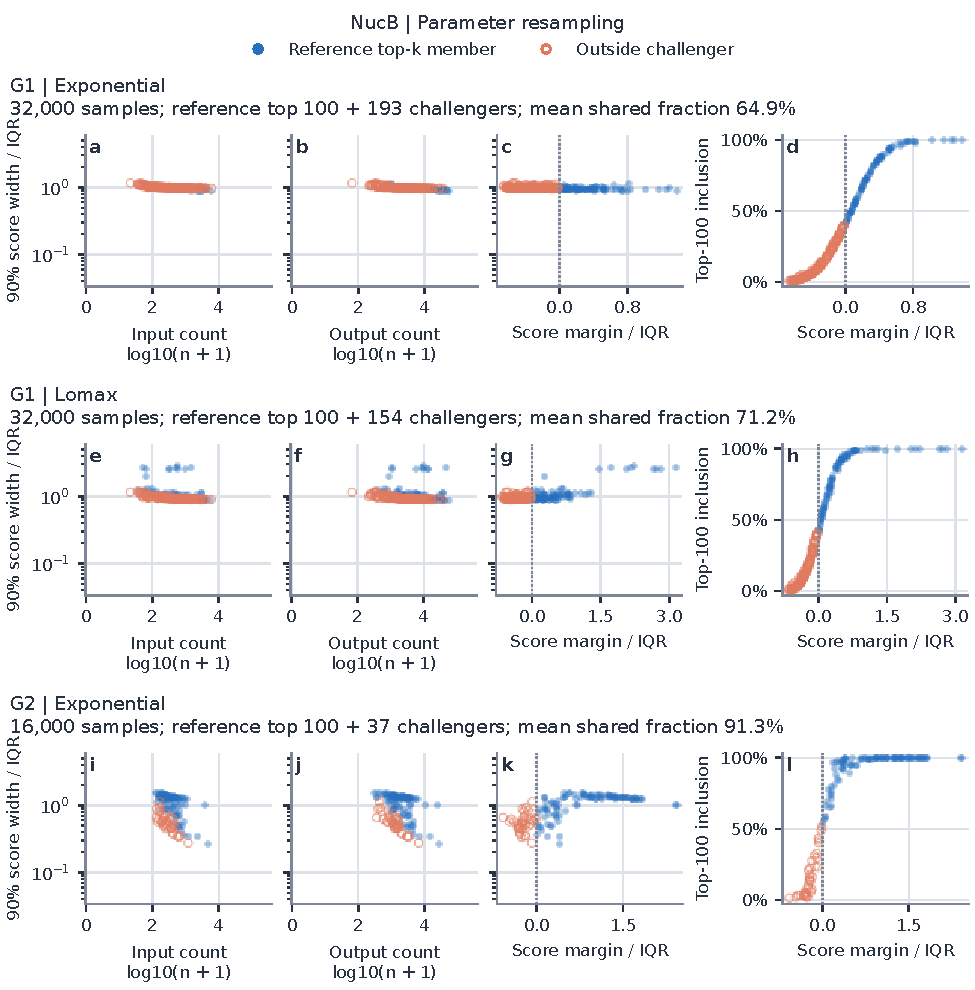
\includegraphics[width=\linewidth]{summary_why_parameter_posterior_nuc_01.pdf}
\caption{NucB decision-cohort summaries: parameter resampling. Rows, top to bottom: nuc-G1, Exponential; nuc-G1, Lomax; nuc-G2, Exponential. Columns show normalized central 90\% score width versus input count, output count, and median-score margin from the top-100 cutoff; then top-100 inclusion versus that margin. Widths and margins use the run's top-1,000 median-score interquartile range (IQR). Blue filled points are reference top-100 members; orange open points are outside candidates with inclusion probability at least 0.01. Count and score-width limits are shared within family and scheme; margin limits are shared within a row. Dotted lines mark the cutoff. No regression lines are fitted.}
\label{fig:why-parameter_posterior-nuc-1}
\end{figure}
\clearpage

\begin{figure}[p]
\centering
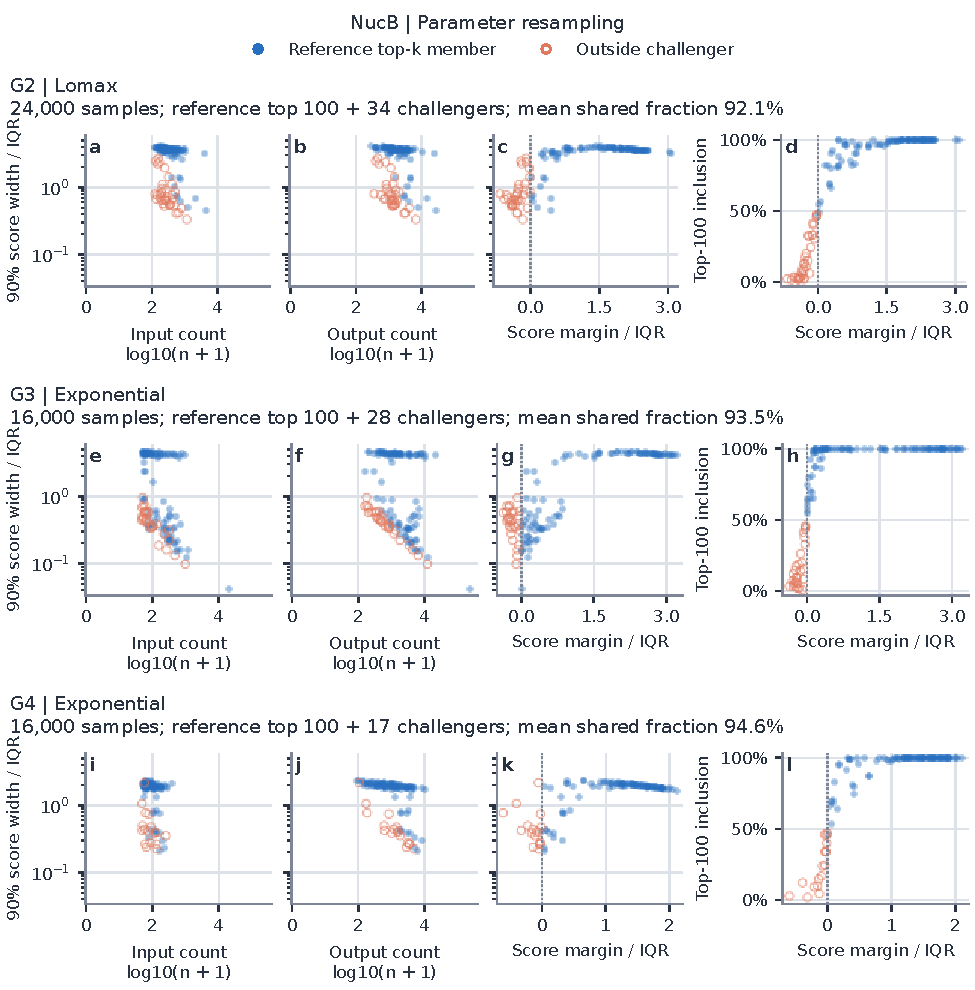
\includegraphics[width=\linewidth]{summary_why_parameter_posterior_nuc_02.pdf}
\caption{NucB decision-cohort summaries: parameter resampling. Rows, top to bottom: nuc-G2, Lomax; nuc-G3, Exponential; nuc-G4, Exponential. Columns show normalized central 90\% score width versus input count, output count, and median-score margin from the top-100 cutoff; then top-100 inclusion versus that margin. Widths and margins use the run's top-1,000 median-score interquartile range (IQR). Blue filled points are reference top-100 members; orange open points are outside candidates with inclusion probability at least 0.01. Count and score-width limits are shared within family and scheme; margin limits are shared within a row. Dotted lines mark the cutoff. No regression lines are fitted.}
\label{fig:why-parameter_posterior-nuc-2}
\end{figure}
\clearpage

\begin{figure}[p]
\centering
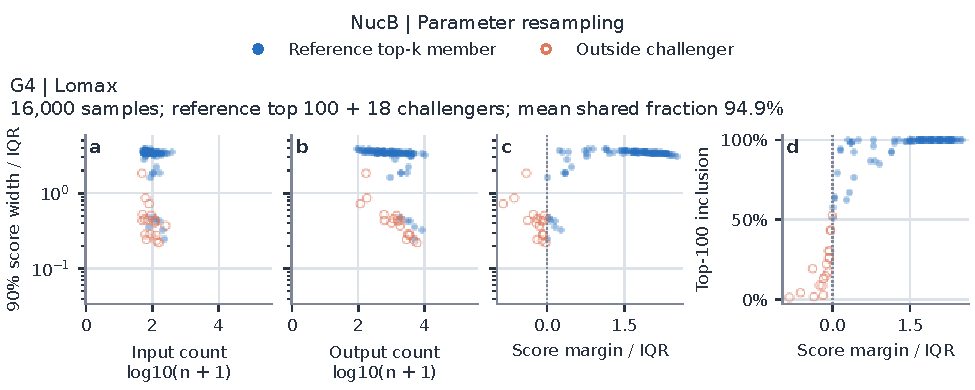
\includegraphics[width=\linewidth]{summary_why_parameter_posterior_nuc_03.pdf}
\caption{NucB decision-cohort summaries: parameter resampling. Rows, top to bottom: nuc-G4, Lomax. Columns show normalized central 90\% score width versus input count, output count, and median-score margin from the top-100 cutoff; then top-100 inclusion versus that margin. Widths and margins use the run's top-1,000 median-score interquartile range (IQR). Blue filled points are reference top-100 members; orange open points are outside candidates with inclusion probability at least 0.01. Count and score-width limits are shared within family and scheme; margin limits are shared within a row. Dotted lines mark the cutoff. No regression lines are fitted.}
\label{fig:why-parameter_posterior-nuc-3}
\end{figure}
\clearpage

\begin{figure}[p]
\centering
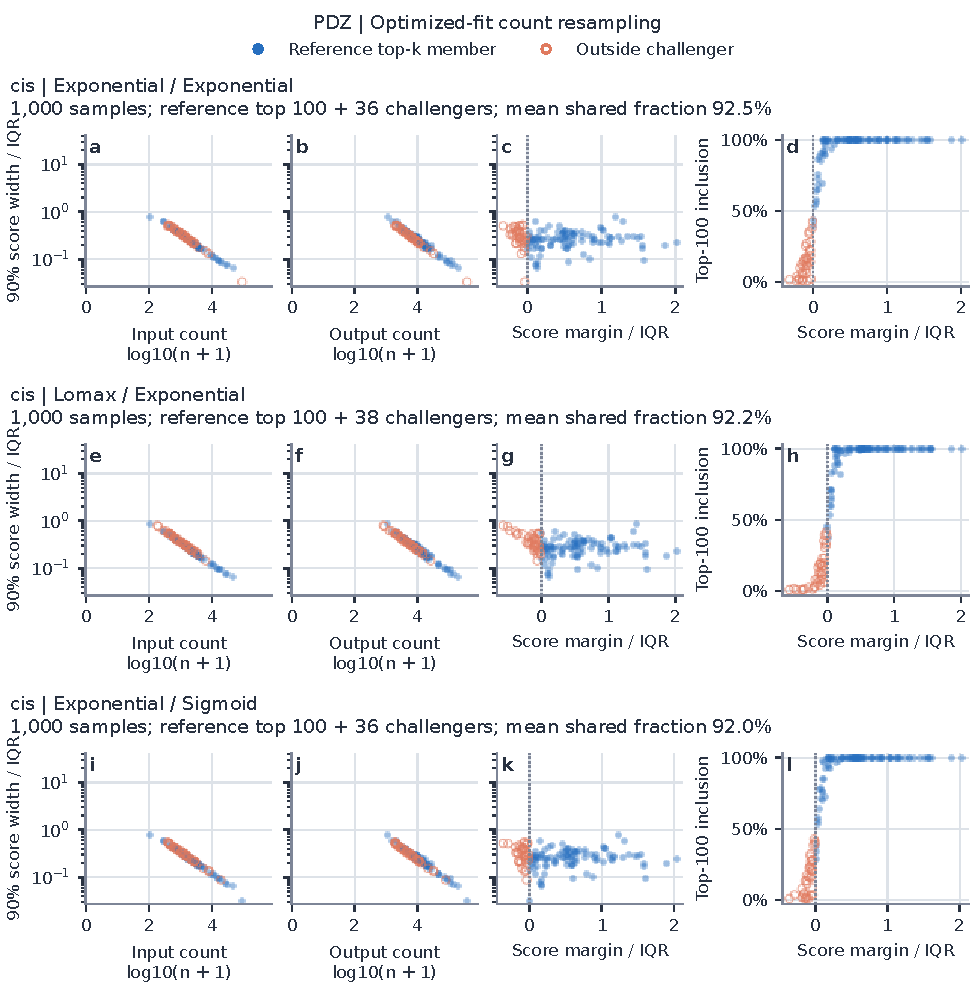
\includegraphics[width=\linewidth]{summary_why_mle_predictive_pdz_01.pdf}
\caption{PDZ decision-cohort summaries: optimized-fit count resampling. Rows, top to bottom: pdz-cis, Exponential--Exponential; pdz-cis, Lomax--Exponential; pdz-cis, Exponential--Sigmoid. Columns show normalized central 90\% score width versus input count, output count, and median-score margin from the top-100 cutoff; then top-100 inclusion versus that margin. Widths and margins use the run's top-1,000 median-score interquartile range (IQR). Blue filled points are reference top-100 members; orange open points are outside candidates with inclusion probability at least 0.01. Count and score-width limits are shared within family and scheme; margin limits are shared within a row. Dotted lines mark the cutoff. No regression lines are fitted.}
\label{fig:why-mle_predictive-pdz-1}
\end{figure}
\clearpage

\begin{figure}[p]
\centering
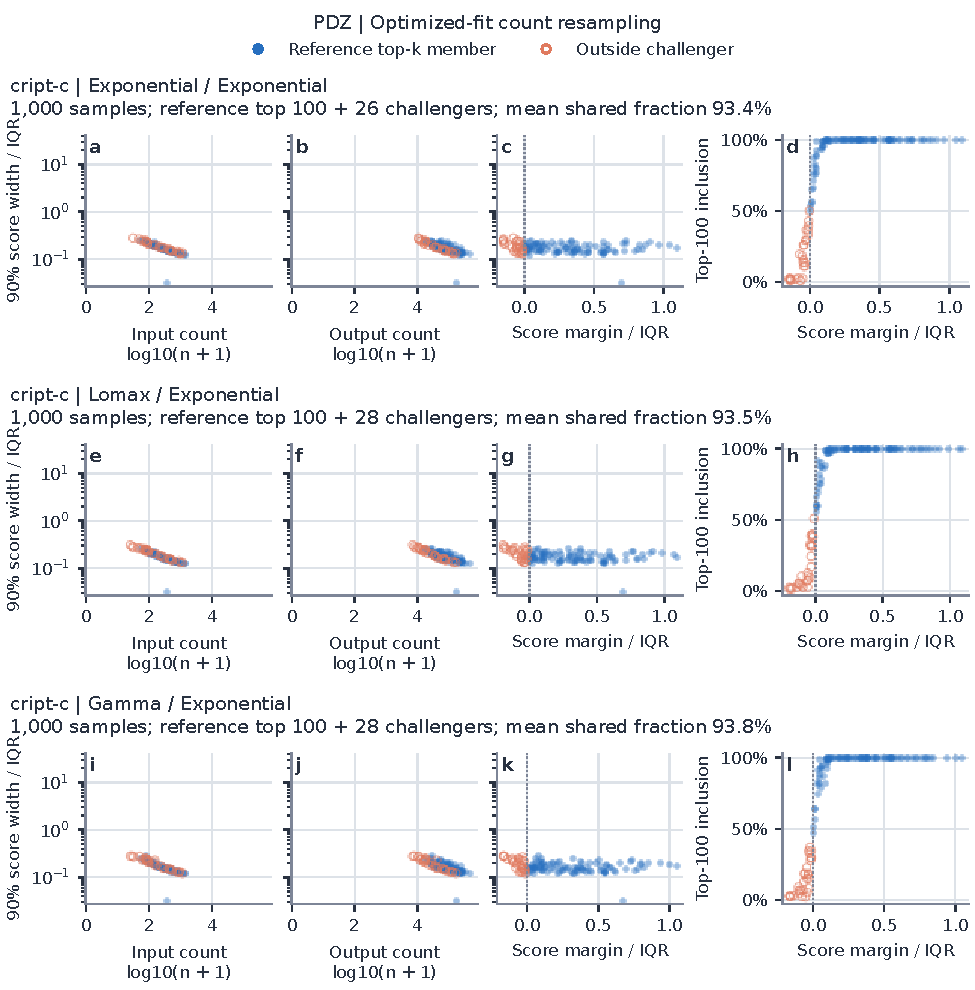
\includegraphics[width=\linewidth]{summary_why_mle_predictive_pdz_02.pdf}
\caption{PDZ decision-cohort summaries: optimized-fit count resampling. Rows, top to bottom: pdz-cript-c, Exponential--Exponential; pdz-cript-c, Lomax--Exponential; pdz-cript-c, Gamma--Exponential. Columns show normalized central 90\% score width versus input count, output count, and median-score margin from the top-100 cutoff; then top-100 inclusion versus that margin. Widths and margins use the run's top-1,000 median-score interquartile range (IQR). Blue filled points are reference top-100 members; orange open points are outside candidates with inclusion probability at least 0.01. Count and score-width limits are shared within family and scheme; margin limits are shared within a row. Dotted lines mark the cutoff. No regression lines are fitted.}
\label{fig:why-mle_predictive-pdz-2}
\end{figure}
\clearpage

\begin{figure}[p]
\centering
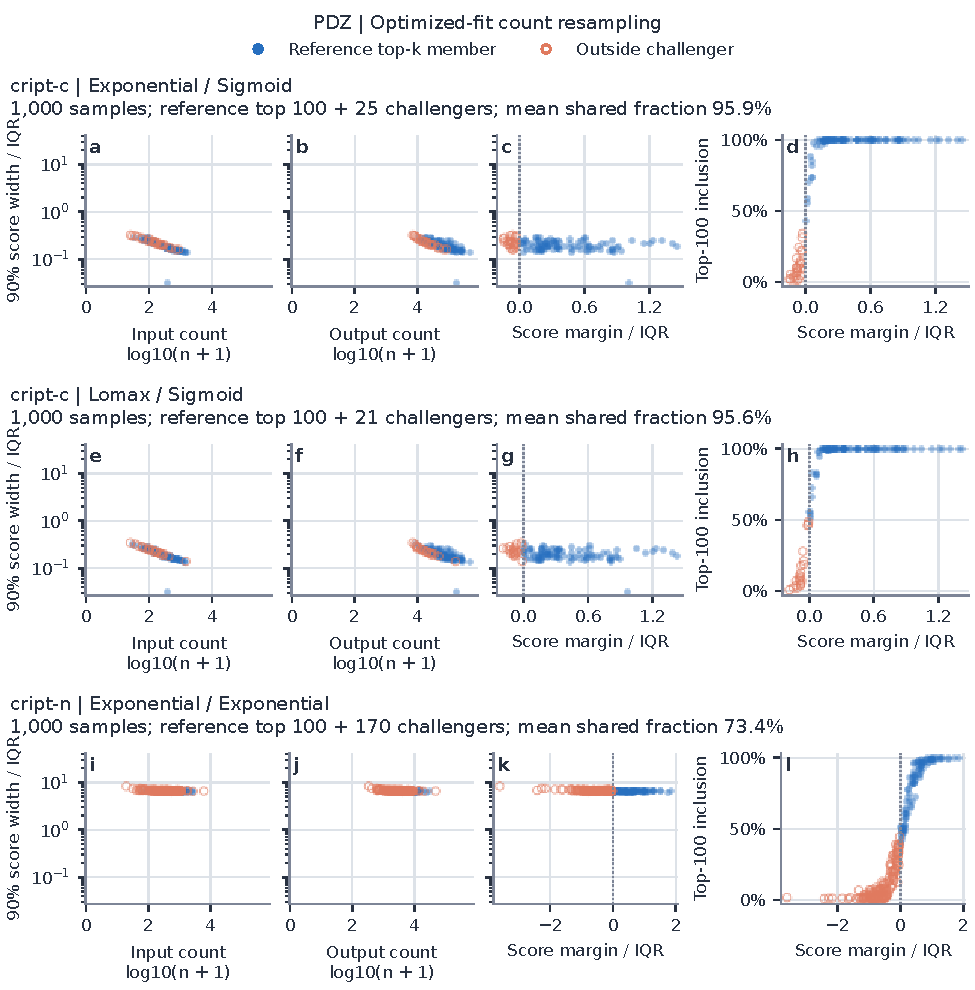
\includegraphics[width=\linewidth]{summary_why_mle_predictive_pdz_03.pdf}
\caption{PDZ decision-cohort summaries: optimized-fit count resampling. Rows, top to bottom: pdz-cript-c, Exponential--Sigmoid; pdz-cript-c, Lomax--Sigmoid; pdz-cript-n, Exponential--Exponential. Columns show normalized central 90\% score width versus input count, output count, and median-score margin from the top-100 cutoff; then top-100 inclusion versus that margin. Widths and margins use the run's top-1,000 median-score interquartile range (IQR). Blue filled points are reference top-100 members; orange open points are outside candidates with inclusion probability at least 0.01. Count and score-width limits are shared within family and scheme; margin limits are shared within a row. Dotted lines mark the cutoff. No regression lines are fitted.}
\label{fig:why-mle_predictive-pdz-3}
\end{figure}
\clearpage

\begin{figure}[p]
\centering
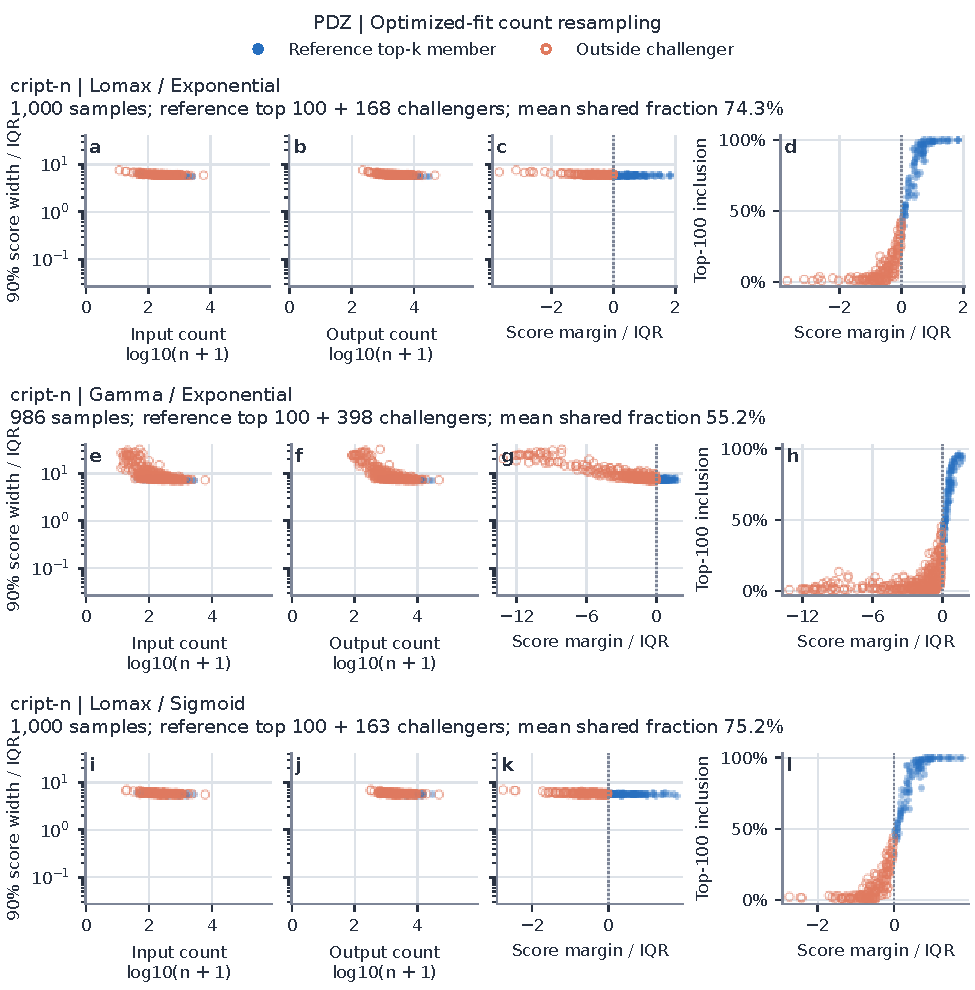
\includegraphics[width=\linewidth]{summary_why_mle_predictive_pdz_04.pdf}
\caption{PDZ decision-cohort summaries: optimized-fit count resampling. Rows, top to bottom: pdz-cript-n, Lomax--Exponential; pdz-cript-n, Gamma--Exponential; pdz-cript-n, Lomax--Sigmoid. Columns show normalized central 90\% score width versus input count, output count, and median-score margin from the top-100 cutoff; then top-100 inclusion versus that margin. Widths and margins use the run's top-1,000 median-score interquartile range (IQR). Blue filled points are reference top-100 members; orange open points are outside candidates with inclusion probability at least 0.01. Count and score-width limits are shared within family and scheme; margin limits are shared within a row. Dotted lines mark the cutoff. No regression lines are fitted.}
\label{fig:why-mle_predictive-pdz-4}
\end{figure}
\clearpage

\begin{figure}[p]
\centering
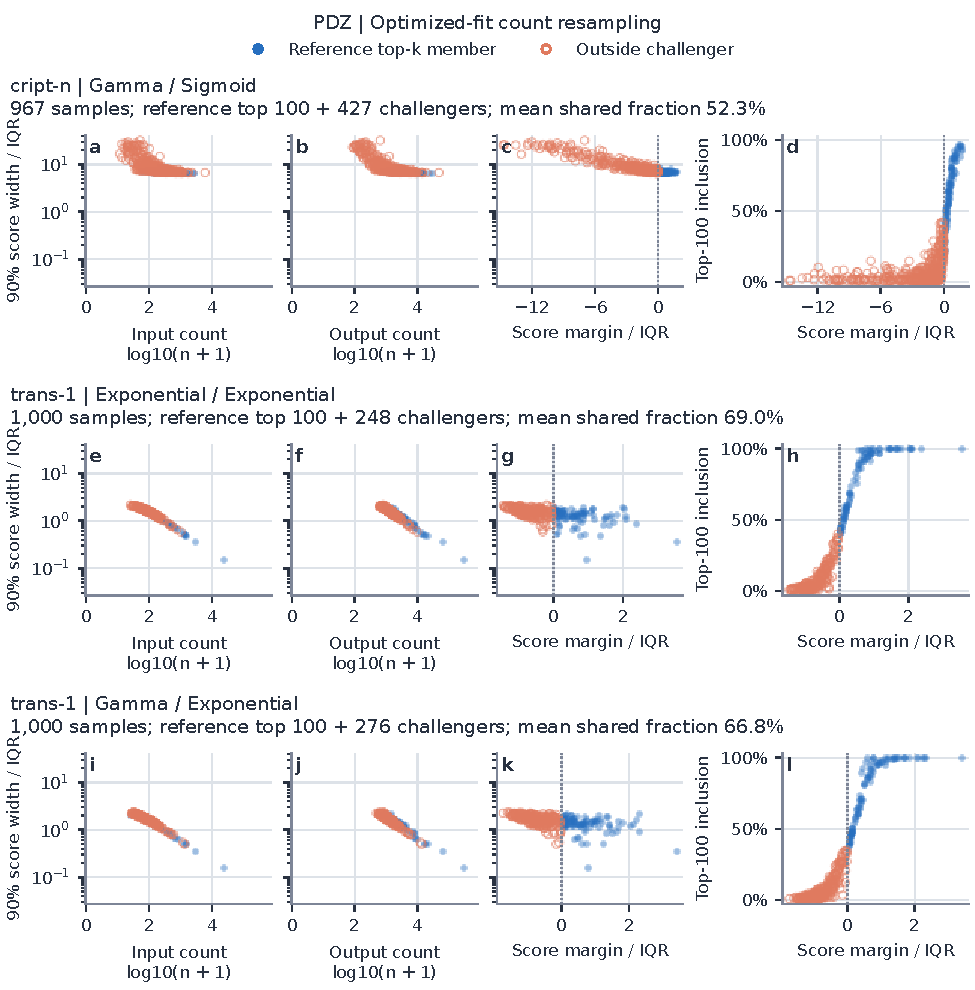
\includegraphics[width=\linewidth]{summary_why_mle_predictive_pdz_05.pdf}
\caption{PDZ decision-cohort summaries: optimized-fit count resampling. Rows, top to bottom: pdz-cript-n, Gamma--Sigmoid; pdz-trans-1, Exponential--Exponential; pdz-trans-1, Gamma--Exponential. Columns show normalized central 90\% score width versus input count, output count, and median-score margin from the top-100 cutoff; then top-100 inclusion versus that margin. Widths and margins use the run's top-1,000 median-score interquartile range (IQR). Blue filled points are reference top-100 members; orange open points are outside candidates with inclusion probability at least 0.01. Count and score-width limits are shared within family and scheme; margin limits are shared within a row. Dotted lines mark the cutoff. No regression lines are fitted.}
\label{fig:why-mle_predictive-pdz-5}
\end{figure}
\clearpage

\begin{figure}[p]
\centering
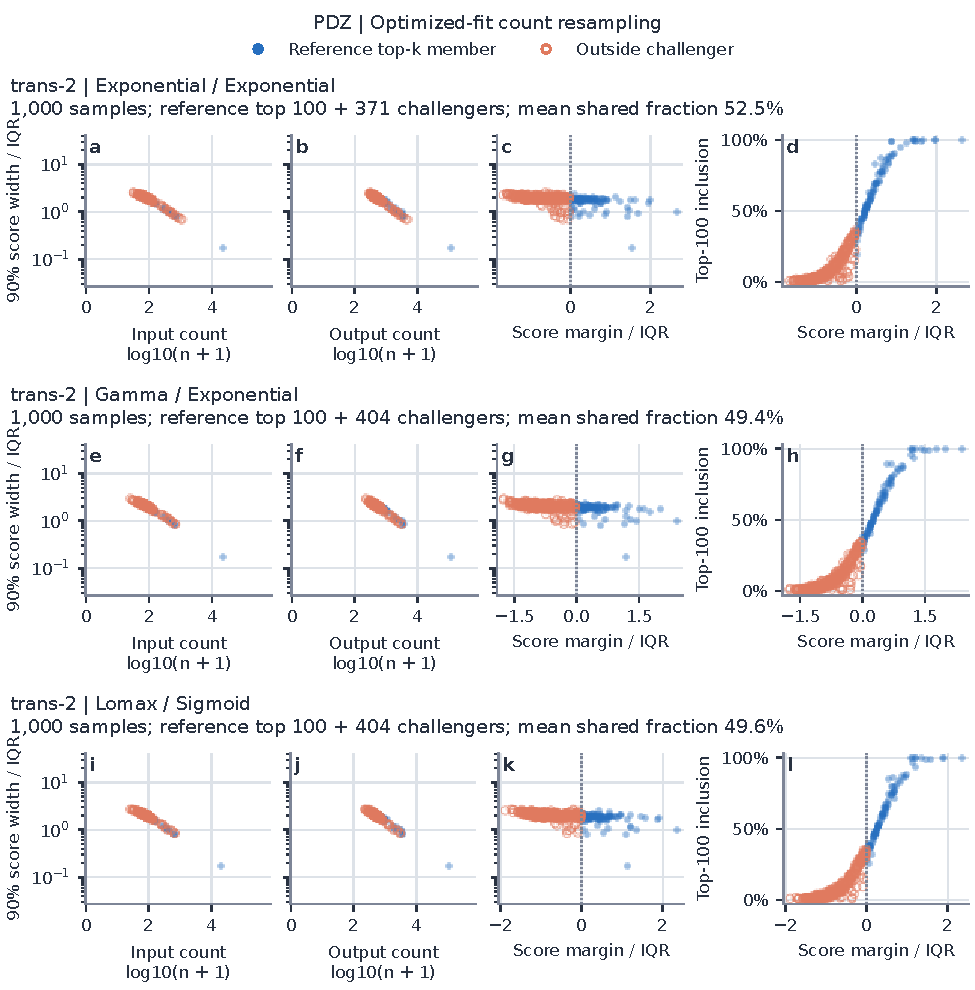
\includegraphics[width=\linewidth]{summary_why_mle_predictive_pdz_06.pdf}
\caption{PDZ decision-cohort summaries: optimized-fit count resampling. Rows, top to bottom: pdz-trans-2, Exponential--Exponential; pdz-trans-2, Gamma--Exponential; pdz-trans-2, Lomax--Sigmoid. Columns show normalized central 90\% score width versus input count, output count, and median-score margin from the top-100 cutoff; then top-100 inclusion versus that margin. Widths and margins use the run's top-1,000 median-score interquartile range (IQR). Blue filled points are reference top-100 members; orange open points are outside candidates with inclusion probability at least 0.01. Count and score-width limits are shared within family and scheme; margin limits are shared within a row. Dotted lines mark the cutoff. No regression lines are fitted.}
\label{fig:why-mle_predictive-pdz-6}
\end{figure}
\clearpage

\begin{figure}[p]
\centering
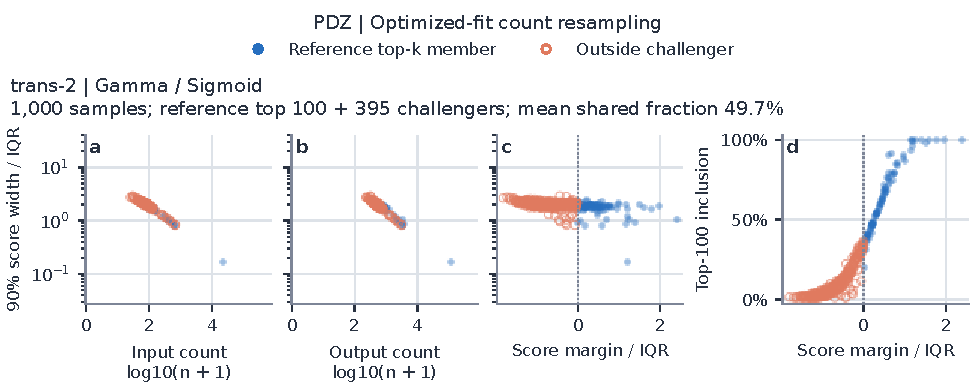
\includegraphics[width=\linewidth]{summary_why_mle_predictive_pdz_07.pdf}
\caption{PDZ decision-cohort summaries: optimized-fit count resampling. Rows, top to bottom: pdz-trans-2, Gamma--Sigmoid. Columns show normalized central 90\% score width versus input count, output count, and median-score margin from the top-100 cutoff; then top-100 inclusion versus that margin. Widths and margins use the run's top-1,000 median-score interquartile range (IQR). Blue filled points are reference top-100 members; orange open points are outside candidates with inclusion probability at least 0.01. Count and score-width limits are shared within family and scheme; margin limits are shared within a row. Dotted lines mark the cutoff. No regression lines are fitted.}
\label{fig:why-mle_predictive-pdz-7}
\end{figure}
\clearpage

\begin{figure}[p]
\centering
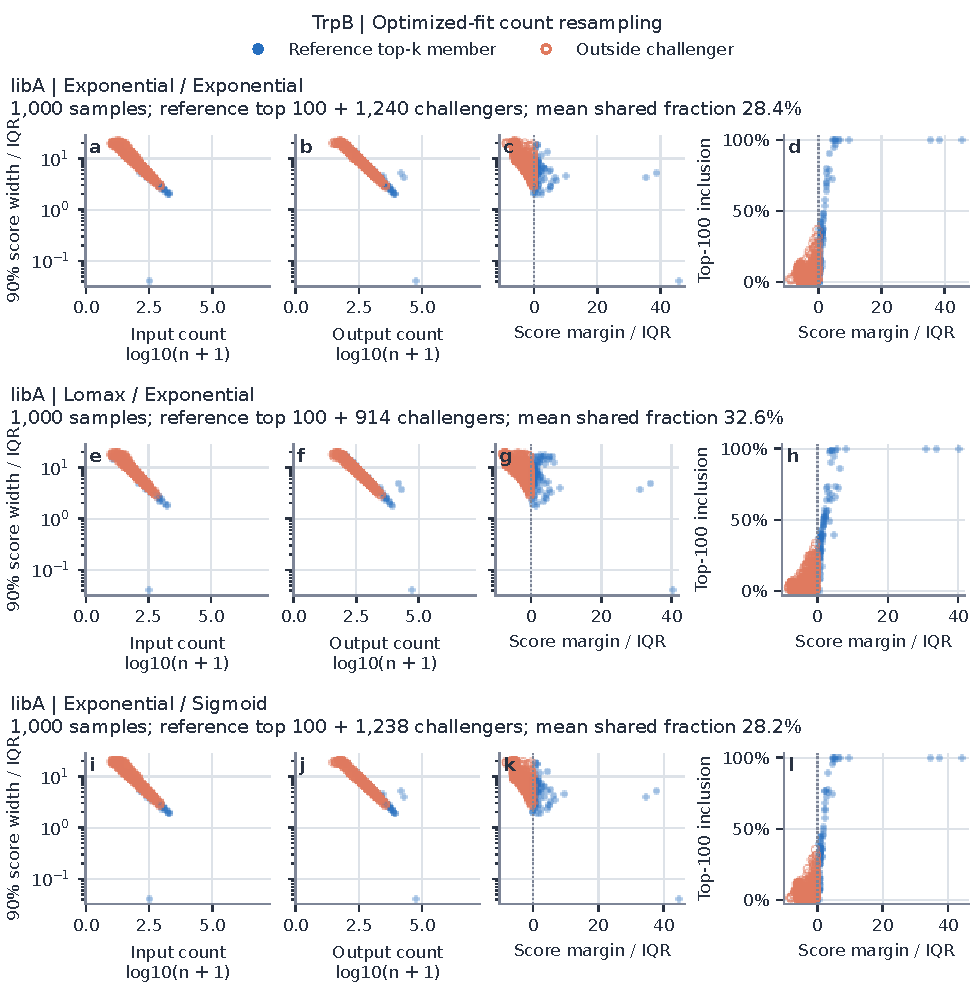
\includegraphics[width=\linewidth]{summary_why_mle_predictive_trpb_01.pdf}
\caption{TrpB decision-cohort summaries: optimized-fit count resampling. Rows, top to bottom: trpb-libA, Exponential--Exponential; trpb-libA, Lomax--Exponential; trpb-libA, Exponential--Sigmoid. Columns show normalized central 90\% score width versus input count, output count, and median-score margin from the top-100 cutoff; then top-100 inclusion versus that margin. Widths and margins use the run's top-1,000 median-score interquartile range (IQR). Blue filled points are reference top-100 members; orange open points are outside candidates with inclusion probability at least 0.01. Count and score-width limits are shared within family and scheme; margin limits are shared within a row. Dotted lines mark the cutoff. No regression lines are fitted.}
\label{fig:why-mle_predictive-trpb-1}
\end{figure}
\clearpage

\begin{figure}[p]
\centering
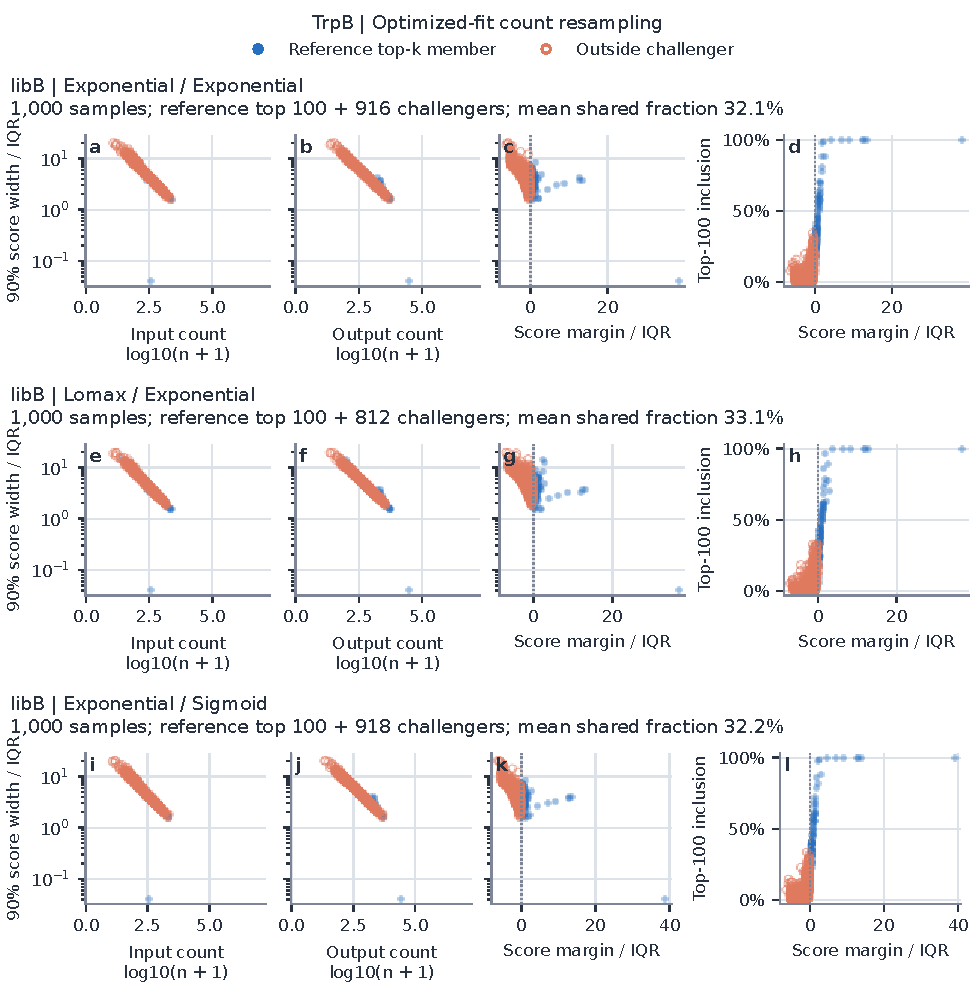
\includegraphics[width=\linewidth]{summary_why_mle_predictive_trpb_02.pdf}
\caption{TrpB decision-cohort summaries: optimized-fit count resampling. Rows, top to bottom: trpb-libB, Exponential--Exponential; trpb-libB, Lomax--Exponential; trpb-libB, Exponential--Sigmoid. Columns show normalized central 90\% score width versus input count, output count, and median-score margin from the top-100 cutoff; then top-100 inclusion versus that margin. Widths and margins use the run's top-1,000 median-score interquartile range (IQR). Blue filled points are reference top-100 members; orange open points are outside candidates with inclusion probability at least 0.01. Count and score-width limits are shared within family and scheme; margin limits are shared within a row. Dotted lines mark the cutoff. No regression lines are fitted.}
\label{fig:why-mle_predictive-trpb-2}
\end{figure}
\clearpage

\begin{figure}[p]
\centering
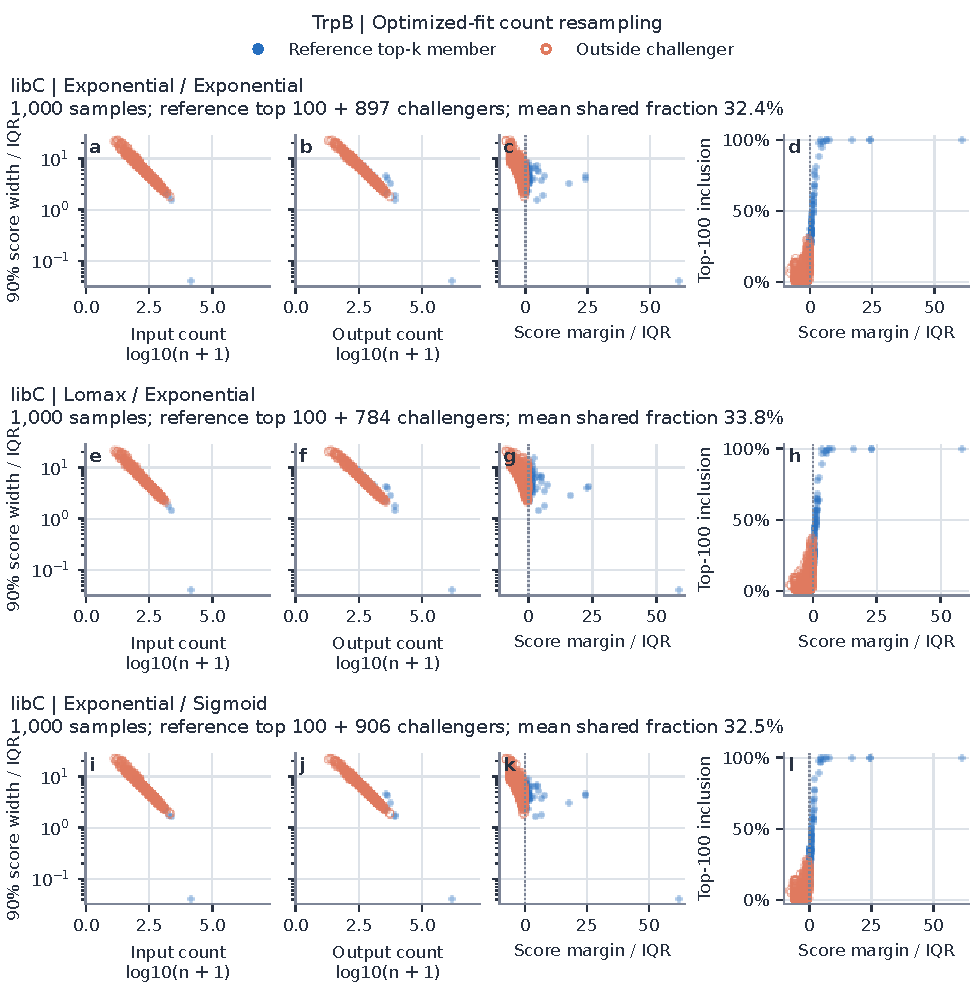
\includegraphics[width=\linewidth]{summary_why_mle_predictive_trpb_03.pdf}
\caption{TrpB decision-cohort summaries: optimized-fit count resampling. Rows, top to bottom: trpb-libC, Exponential--Exponential; trpb-libC, Lomax--Exponential; trpb-libC, Exponential--Sigmoid. Columns show normalized central 90\% score width versus input count, output count, and median-score margin from the top-100 cutoff; then top-100 inclusion versus that margin. Widths and margins use the run's top-1,000 median-score interquartile range (IQR). Blue filled points are reference top-100 members; orange open points are outside candidates with inclusion probability at least 0.01. Count and score-width limits are shared within family and scheme; margin limits are shared within a row. Dotted lines mark the cutoff. No regression lines are fitted.}
\label{fig:why-mle_predictive-trpb-3}
\end{figure}
\clearpage

\begin{figure}[p]
\centering
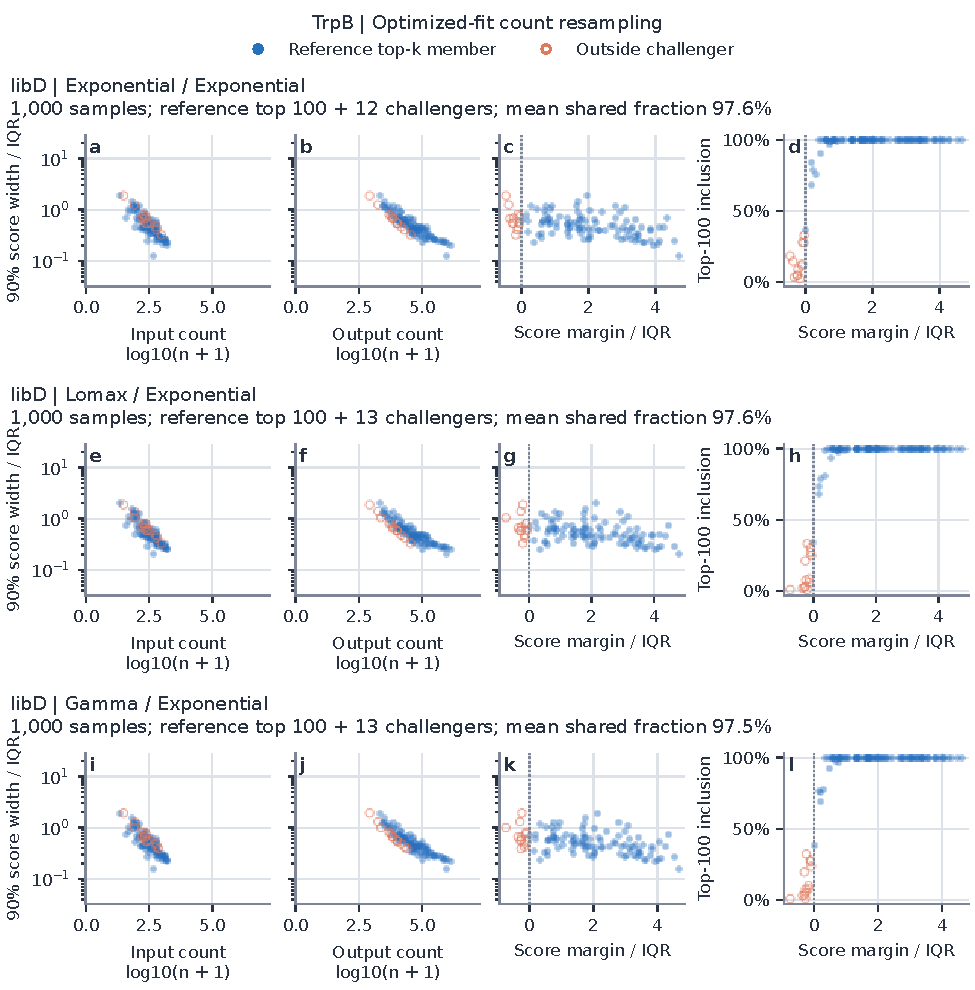
\includegraphics[width=\linewidth]{summary_why_mle_predictive_trpb_04.pdf}
\caption{TrpB decision-cohort summaries: optimized-fit count resampling. Rows, top to bottom: trpb-libD, Exponential--Exponential; trpb-libD, Lomax--Exponential; trpb-libD, Gamma--Exponential. Columns show normalized central 90\% score width versus input count, output count, and median-score margin from the top-100 cutoff; then top-100 inclusion versus that margin. Widths and margins use the run's top-1,000 median-score interquartile range (IQR). Blue filled points are reference top-100 members; orange open points are outside candidates with inclusion probability at least 0.01. Count and score-width limits are shared within family and scheme; margin limits are shared within a row. Dotted lines mark the cutoff. No regression lines are fitted.}
\label{fig:why-mle_predictive-trpb-4}
\end{figure}
\clearpage

\begin{figure}[p]
\centering
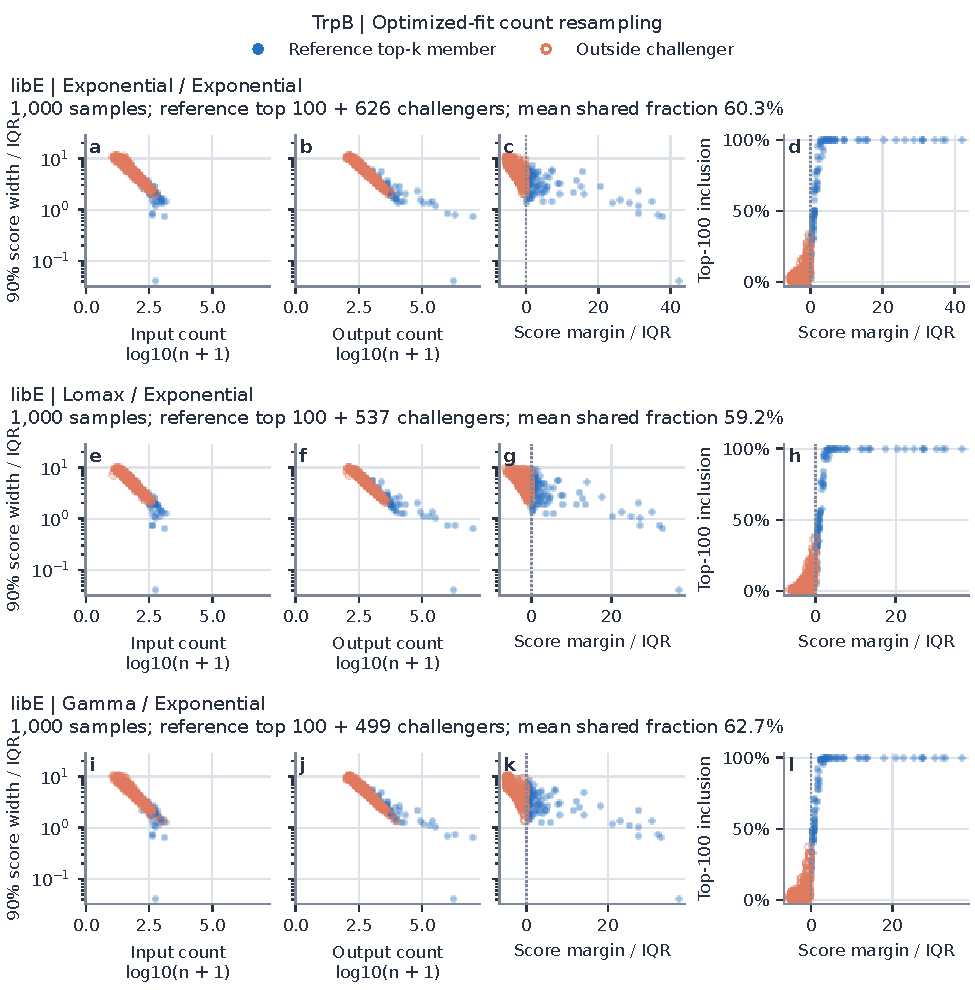
\includegraphics[width=\linewidth]{summary_why_mle_predictive_trpb_05.pdf}
\caption{TrpB decision-cohort summaries: optimized-fit count resampling. Rows, top to bottom: trpb-libE, Exponential--Exponential; trpb-libE, Lomax--Exponential; trpb-libE, Gamma--Exponential. Columns show normalized central 90\% score width versus input count, output count, and median-score margin from the top-100 cutoff; then top-100 inclusion versus that margin. Widths and margins use the run's top-1,000 median-score interquartile range (IQR). Blue filled points are reference top-100 members; orange open points are outside candidates with inclusion probability at least 0.01. Count and score-width limits are shared within family and scheme; margin limits are shared within a row. Dotted lines mark the cutoff. No regression lines are fitted.}
\label{fig:why-mle_predictive-trpb-5}
\end{figure}
\clearpage

\begin{figure}[p]
\centering
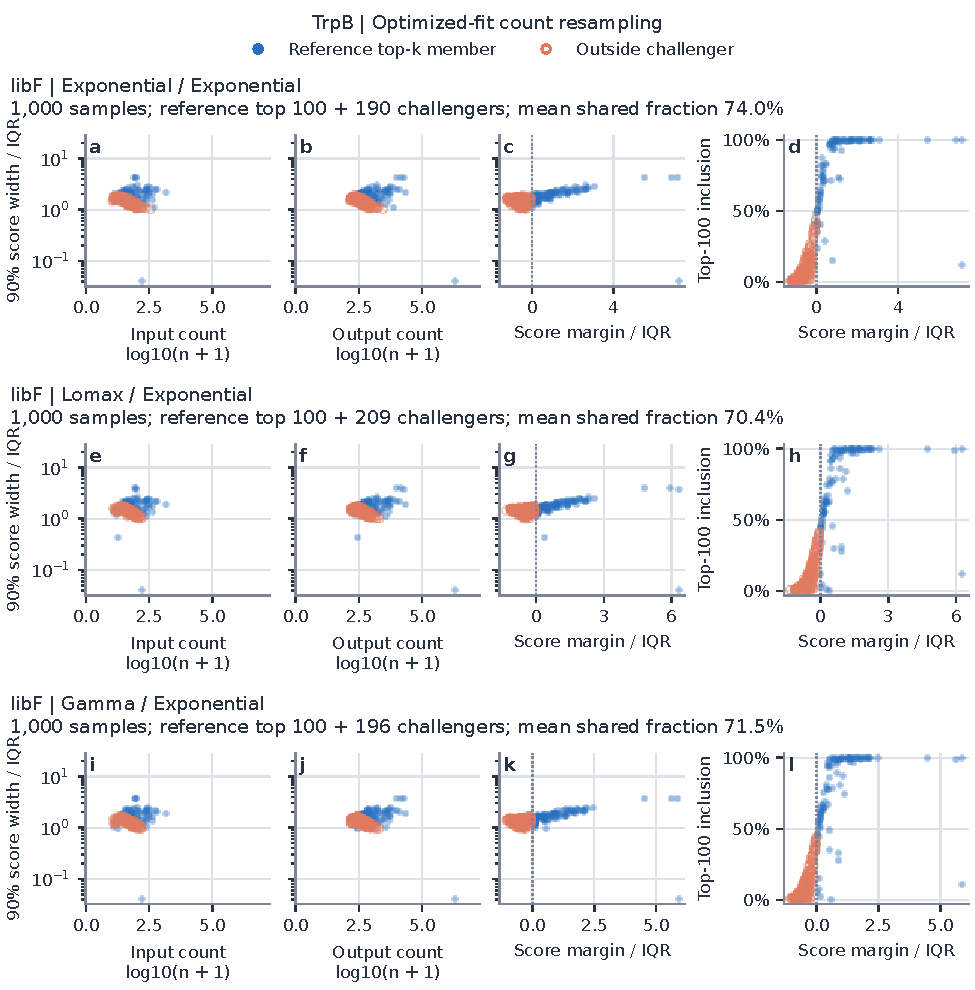
\includegraphics[width=\linewidth]{summary_why_mle_predictive_trpb_06.pdf}
\caption{TrpB decision-cohort summaries: optimized-fit count resampling. Rows, top to bottom: trpb-libF, Exponential--Exponential; trpb-libF, Lomax--Exponential; trpb-libF, Gamma--Exponential. Columns show normalized central 90\% score width versus input count, output count, and median-score margin from the top-100 cutoff; then top-100 inclusion versus that margin. Widths and margins use the run's top-1,000 median-score interquartile range (IQR). Blue filled points are reference top-100 members; orange open points are outside candidates with inclusion probability at least 0.01. Count and score-width limits are shared within family and scheme; margin limits are shared within a row. Dotted lines mark the cutoff. No regression lines are fitted.}
\label{fig:why-mle_predictive-trpb-6}
\end{figure}
\clearpage

\begin{figure}[p]
\centering
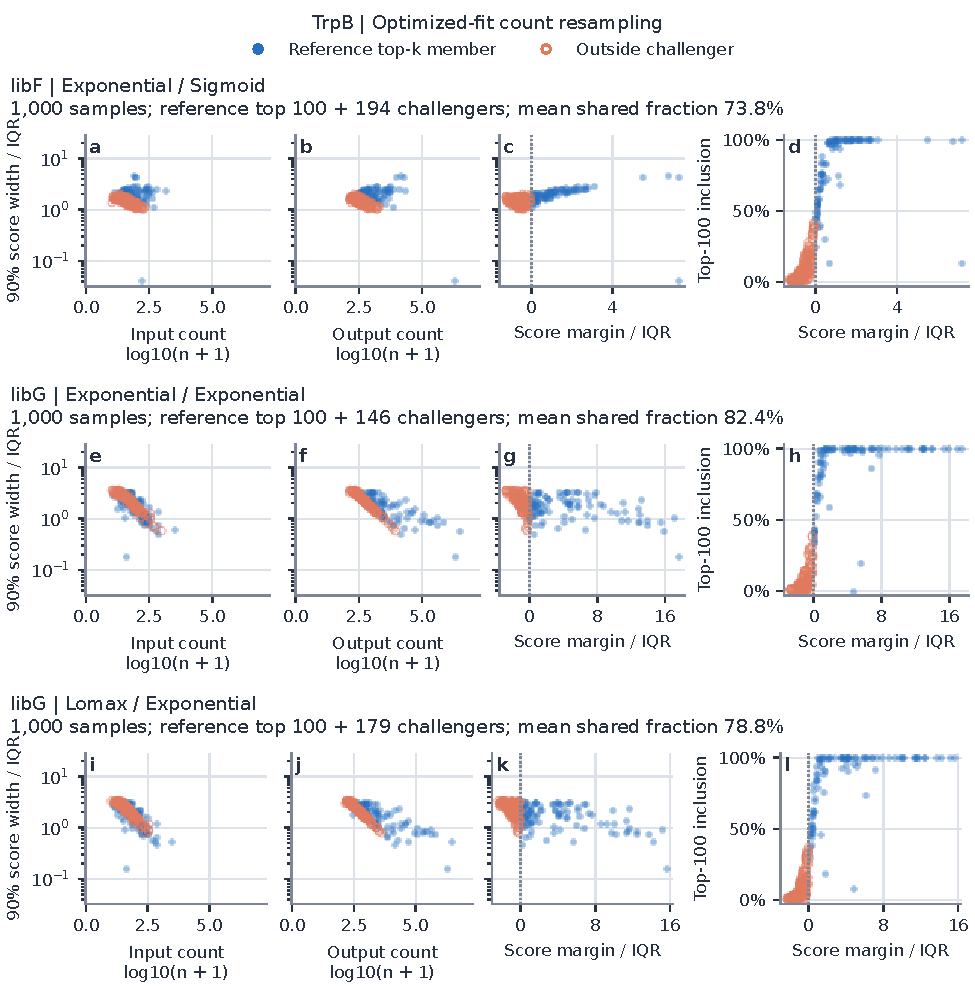
\includegraphics[width=\linewidth]{summary_why_mle_predictive_trpb_07.pdf}
\caption{TrpB decision-cohort summaries: optimized-fit count resampling. Rows, top to bottom: trpb-libF, Exponential--Sigmoid; trpb-libG, Exponential--Exponential; trpb-libG, Lomax--Exponential. Columns show normalized central 90\% score width versus input count, output count, and median-score margin from the top-100 cutoff; then top-100 inclusion versus that margin. Widths and margins use the run's top-1,000 median-score interquartile range (IQR). Blue filled points are reference top-100 members; orange open points are outside candidates with inclusion probability at least 0.01. Count and score-width limits are shared within family and scheme; margin limits are shared within a row. Dotted lines mark the cutoff. No regression lines are fitted.}
\label{fig:why-mle_predictive-trpb-7}
\end{figure}
\clearpage

\begin{figure}[p]
\centering
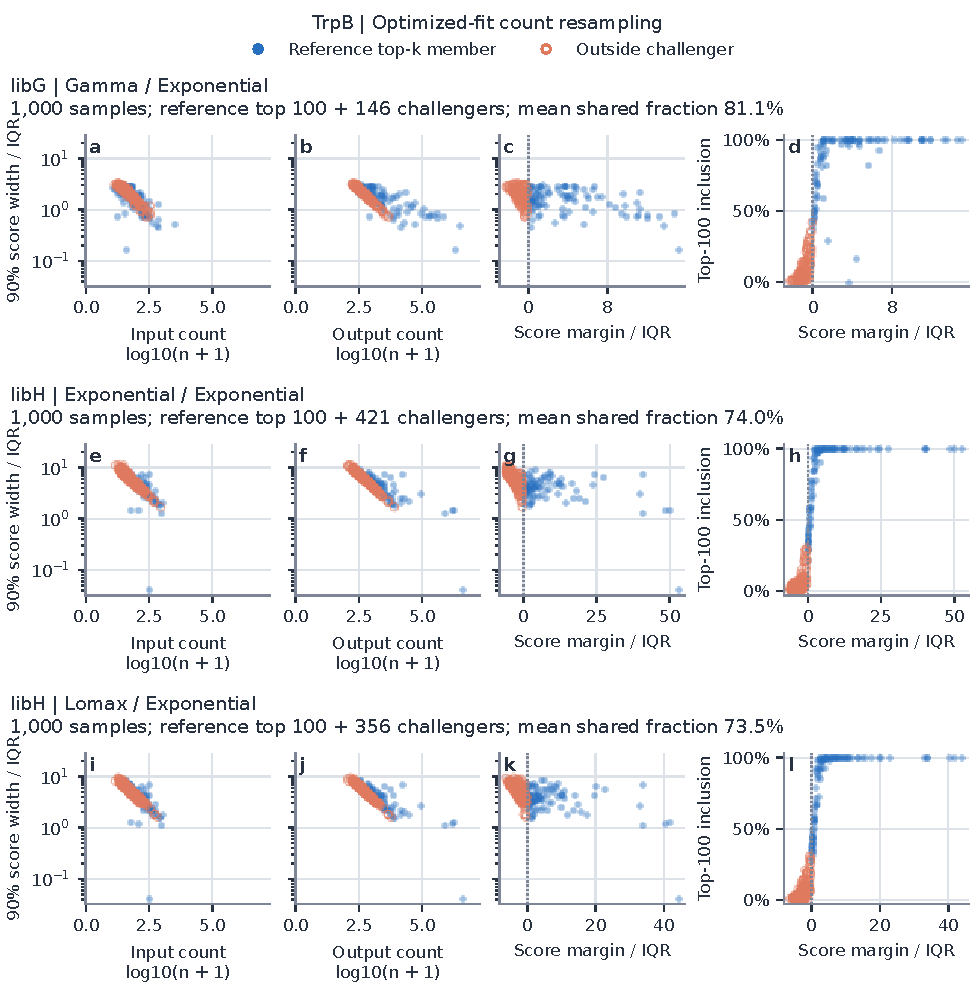
\includegraphics[width=\linewidth]{summary_why_mle_predictive_trpb_08.pdf}
\caption{TrpB decision-cohort summaries: optimized-fit count resampling. Rows, top to bottom: trpb-libG, Gamma--Exponential; trpb-libH, Exponential--Exponential; trpb-libH, Lomax--Exponential. Columns show normalized central 90\% score width versus input count, output count, and median-score margin from the top-100 cutoff; then top-100 inclusion versus that margin. Widths and margins use the run's top-1,000 median-score interquartile range (IQR). Blue filled points are reference top-100 members; orange open points are outside candidates with inclusion probability at least 0.01. Count and score-width limits are shared within family and scheme; margin limits are shared within a row. Dotted lines mark the cutoff. No regression lines are fitted.}
\label{fig:why-mle_predictive-trpb-8}
\end{figure}
\clearpage

\begin{figure}[p]
\centering
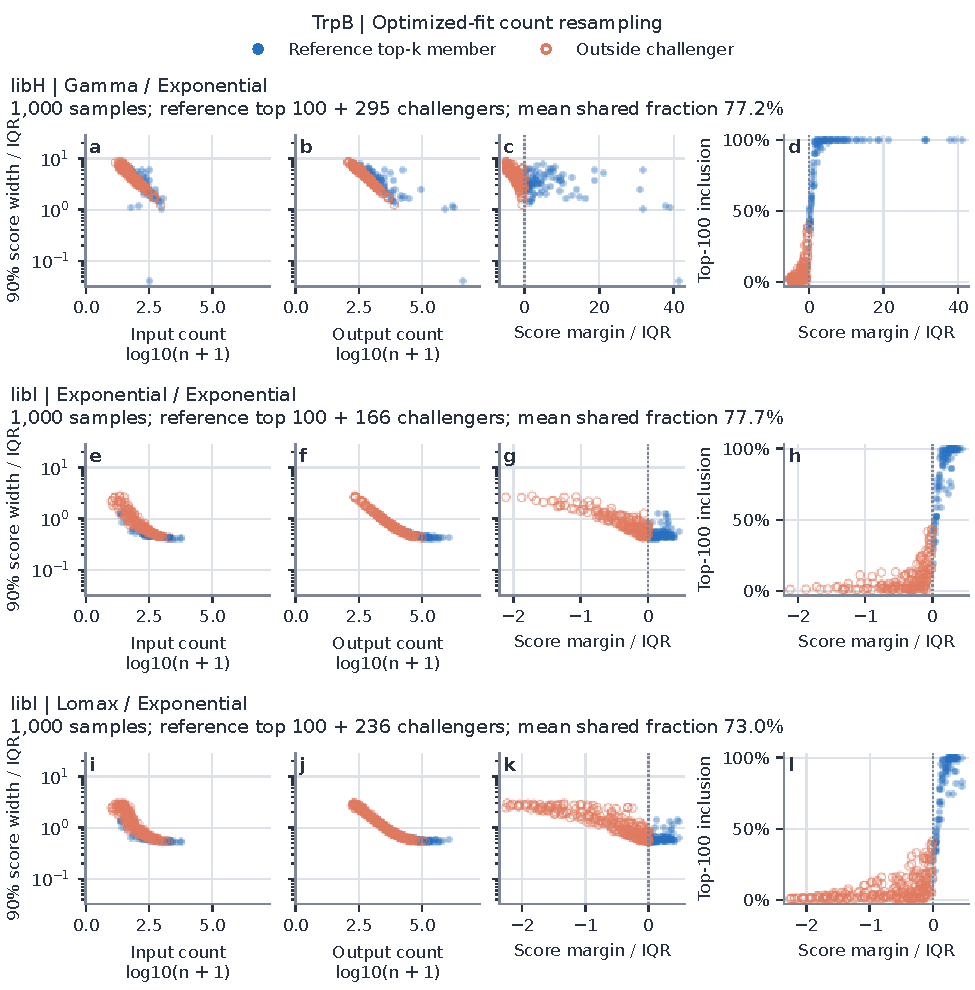
\includegraphics[width=\linewidth]{summary_why_mle_predictive_trpb_09.pdf}
\caption{TrpB decision-cohort summaries: optimized-fit count resampling. Rows, top to bottom: trpb-libH, Gamma--Exponential; trpb-libI, Exponential--Exponential; trpb-libI, Lomax--Exponential. Columns show normalized central 90\% score width versus input count, output count, and median-score margin from the top-100 cutoff; then top-100 inclusion versus that margin. Widths and margins use the run's top-1,000 median-score interquartile range (IQR). Blue filled points are reference top-100 members; orange open points are outside candidates with inclusion probability at least 0.01. Count and score-width limits are shared within family and scheme; margin limits are shared within a row. Dotted lines mark the cutoff. No regression lines are fitted.}
\label{fig:why-mle_predictive-trpb-9}
\end{figure}
\clearpage

\begin{figure}[p]
\centering
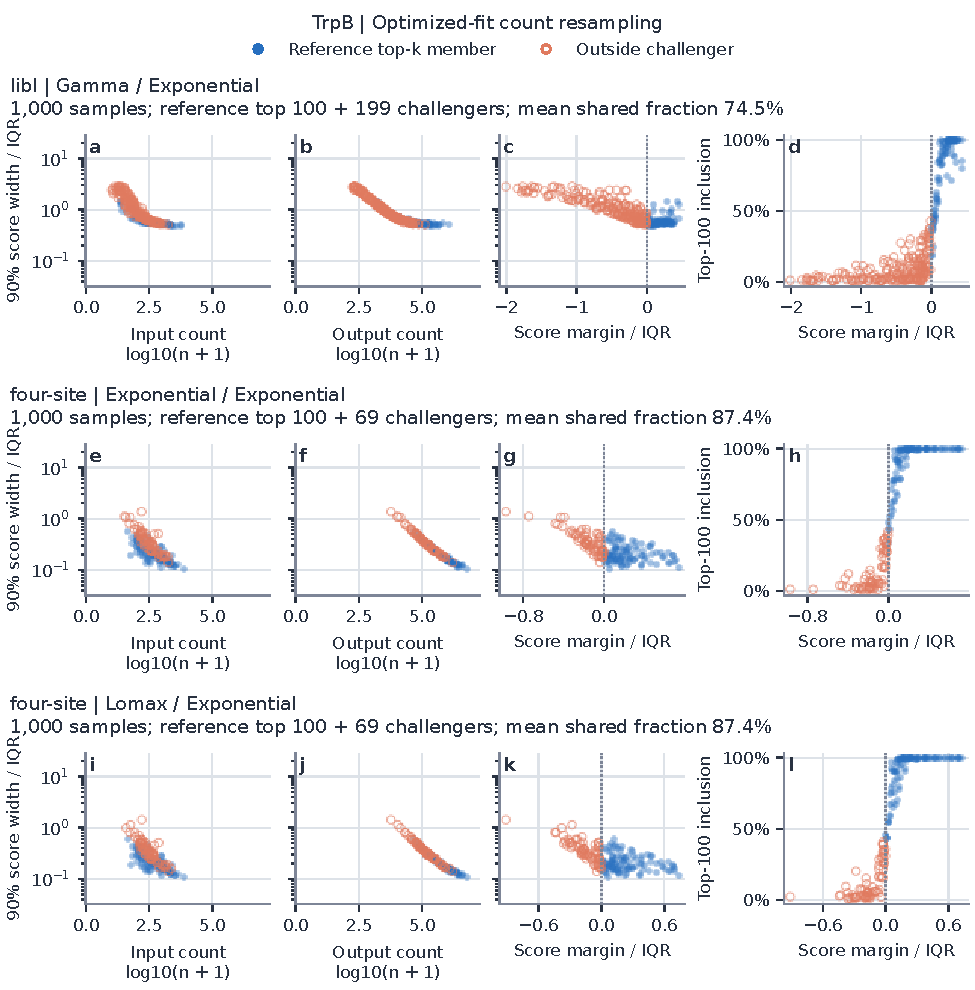
\includegraphics[width=\linewidth]{summary_why_mle_predictive_trpb_10.pdf}
\caption{TrpB decision-cohort summaries: optimized-fit count resampling. Rows, top to bottom: trpb-libI, Gamma--Exponential; trpb-four-site, Exponential--Exponential; trpb-four-site, Lomax--Exponential. Columns show normalized central 90\% score width versus input count, output count, and median-score margin from the top-100 cutoff; then top-100 inclusion versus that margin. Widths and margins use the run's top-1,000 median-score interquartile range (IQR). Blue filled points are reference top-100 members; orange open points are outside candidates with inclusion probability at least 0.01. Count and score-width limits are shared within family and scheme; margin limits are shared within a row. Dotted lines mark the cutoff. No regression lines are fitted.}
\label{fig:why-mle_predictive-trpb-10}
\end{figure}
\clearpage

\begin{figure}[p]
\centering
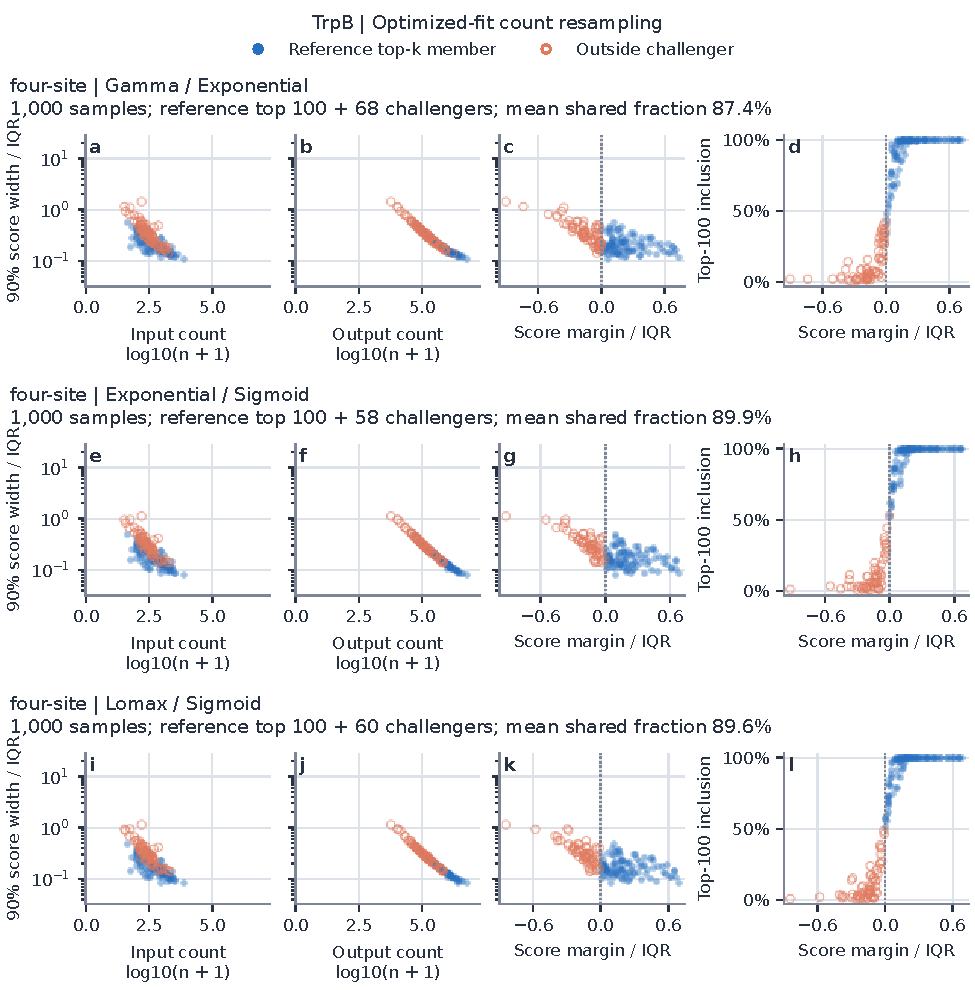
\includegraphics[width=\linewidth]{summary_why_mle_predictive_trpb_11.pdf}
\caption{TrpB decision-cohort summaries: optimized-fit count resampling. Rows, top to bottom: trpb-four-site, Gamma--Exponential; trpb-four-site, Exponential--Sigmoid; trpb-four-site, Lomax--Sigmoid. Columns show normalized central 90\% score width versus input count, output count, and median-score margin from the top-100 cutoff; then top-100 inclusion versus that margin. Widths and margins use the run's top-1,000 median-score interquartile range (IQR). Blue filled points are reference top-100 members; orange open points are outside candidates with inclusion probability at least 0.01. Count and score-width limits are shared within family and scheme; margin limits are shared within a row. Dotted lines mark the cutoff. No regression lines are fitted.}
\label{fig:why-mle_predictive-trpb-11}
\end{figure}
\clearpage

\begin{figure}[p]
\centering
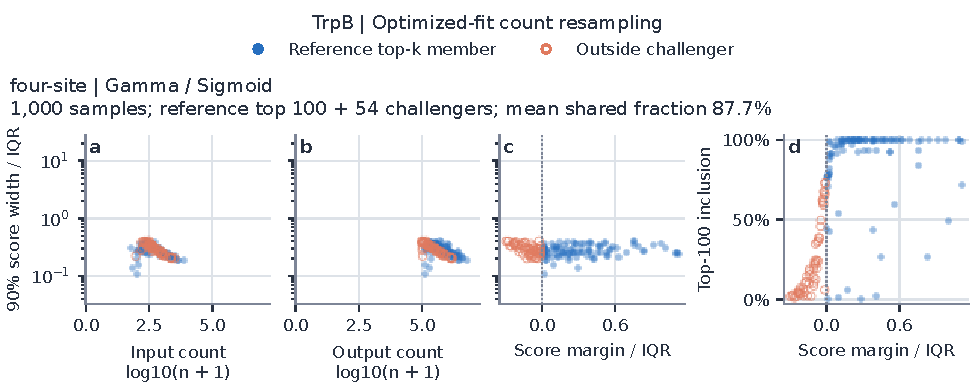
\includegraphics[width=\linewidth]{summary_why_mle_predictive_trpb_12.pdf}
\caption{TrpB decision-cohort summaries: optimized-fit count resampling. Rows, top to bottom: trpb-four-site, Gamma--Sigmoid. Columns show normalized central 90\% score width versus input count, output count, and median-score margin from the top-100 cutoff; then top-100 inclusion versus that margin. Widths and margins use the run's top-1,000 median-score interquartile range (IQR). Blue filled points are reference top-100 members; orange open points are outside candidates with inclusion probability at least 0.01. Count and score-width limits are shared within family and scheme; margin limits are shared within a row. Dotted lines mark the cutoff. No regression lines are fitted.}
\label{fig:why-mle_predictive-trpb-12}
\end{figure}
\clearpage

\begin{figure}[p]
\centering
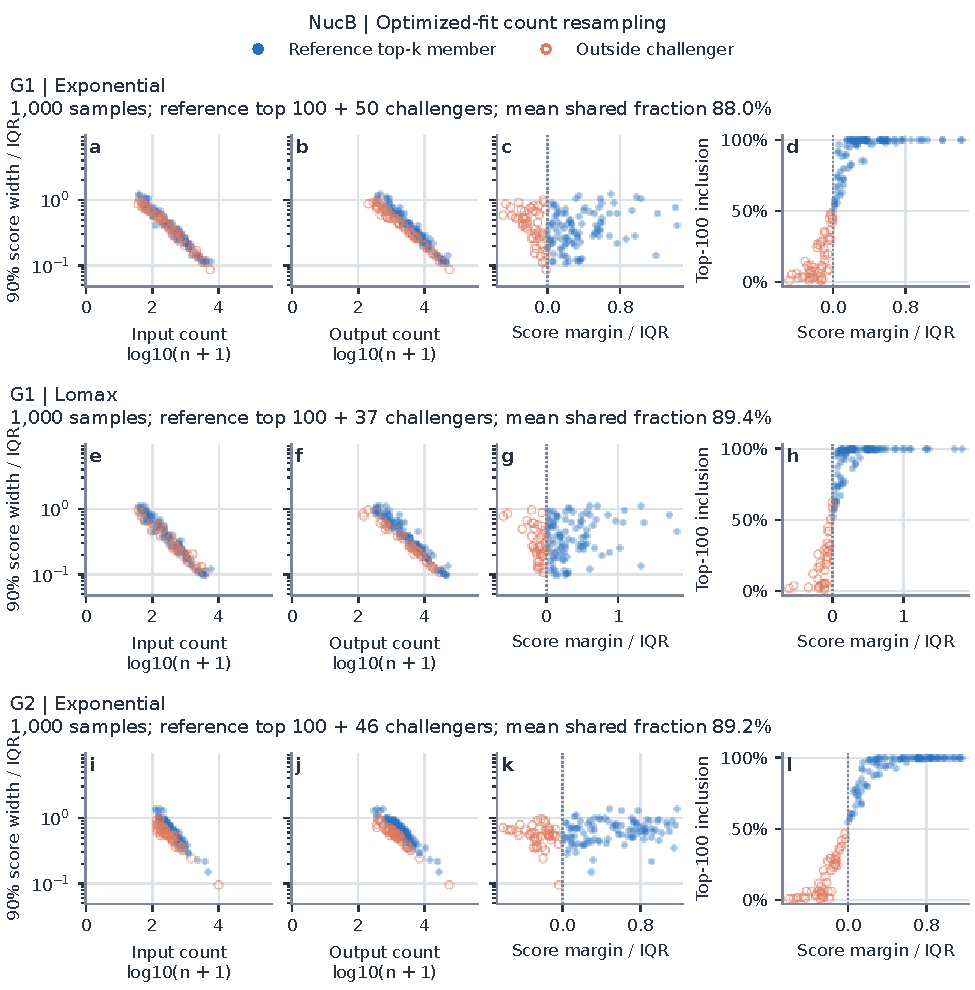
\includegraphics[width=\linewidth]{summary_why_mle_predictive_nuc_01.pdf}
\caption{NucB decision-cohort summaries: optimized-fit count resampling. Rows, top to bottom: nuc-G1, Exponential; nuc-G1, Lomax; nuc-G2, Exponential. Columns show normalized central 90\% score width versus input count, output count, and median-score margin from the top-100 cutoff; then top-100 inclusion versus that margin. Widths and margins use the run's top-1,000 median-score interquartile range (IQR). Blue filled points are reference top-100 members; orange open points are outside candidates with inclusion probability at least 0.01. Count and score-width limits are shared within family and scheme; margin limits are shared within a row. Dotted lines mark the cutoff. No regression lines are fitted.}
\label{fig:why-mle_predictive-nuc-1}
\end{figure}
\clearpage

\begin{figure}[p]
\centering
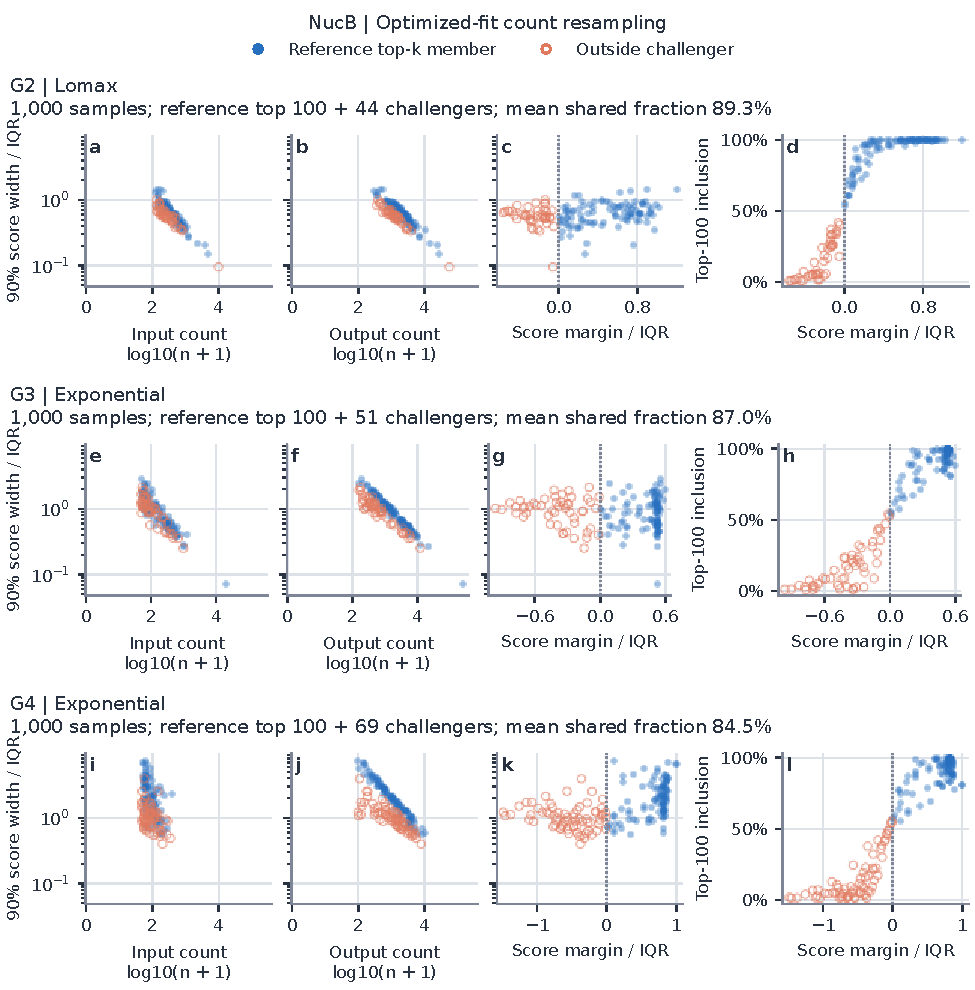
\includegraphics[width=\linewidth]{summary_why_mle_predictive_nuc_02.pdf}
\caption{NucB decision-cohort summaries: optimized-fit count resampling. Rows, top to bottom: nuc-G2, Lomax; nuc-G3, Exponential; nuc-G4, Exponential. Columns show normalized central 90\% score width versus input count, output count, and median-score margin from the top-100 cutoff; then top-100 inclusion versus that margin. Widths and margins use the run's top-1,000 median-score interquartile range (IQR). Blue filled points are reference top-100 members; orange open points are outside candidates with inclusion probability at least 0.01. Count and score-width limits are shared within family and scheme; margin limits are shared within a row. Dotted lines mark the cutoff. No regression lines are fitted.}
\label{fig:why-mle_predictive-nuc-2}
\end{figure}
\clearpage

\begin{figure}[p]
\centering
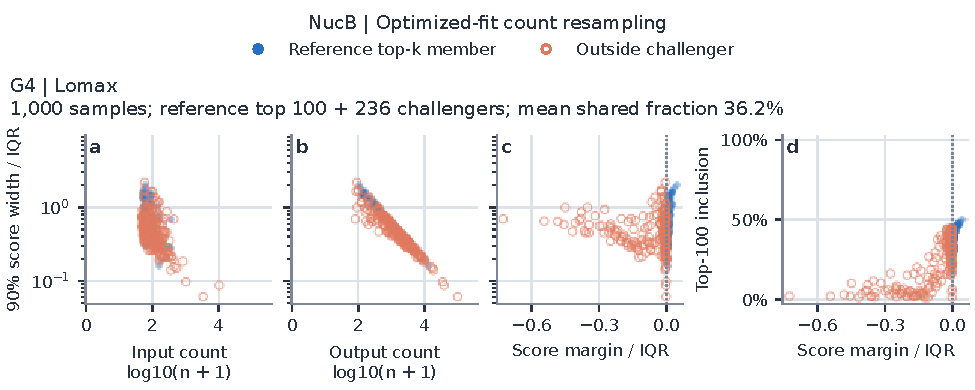
\includegraphics[width=\linewidth]{summary_why_mle_predictive_nuc_03.pdf}
\caption{NucB decision-cohort summaries: optimized-fit count resampling. Rows, top to bottom: nuc-G4, Lomax. Columns show normalized central 90\% score width versus input count, output count, and median-score margin from the top-100 cutoff; then top-100 inclusion versus that margin. Widths and margins use the run's top-1,000 median-score interquartile range (IQR). Blue filled points are reference top-100 members; orange open points are outside candidates with inclusion probability at least 0.01. Count and score-width limits are shared within family and scheme; margin limits are shared within a row. Dotted lines mark the cutoff. No regression lines are fitted.}
\label{fig:why-mle_predictive-nuc-3}
\end{figure}
\clearpage

\begin{figure}[p]
\centering
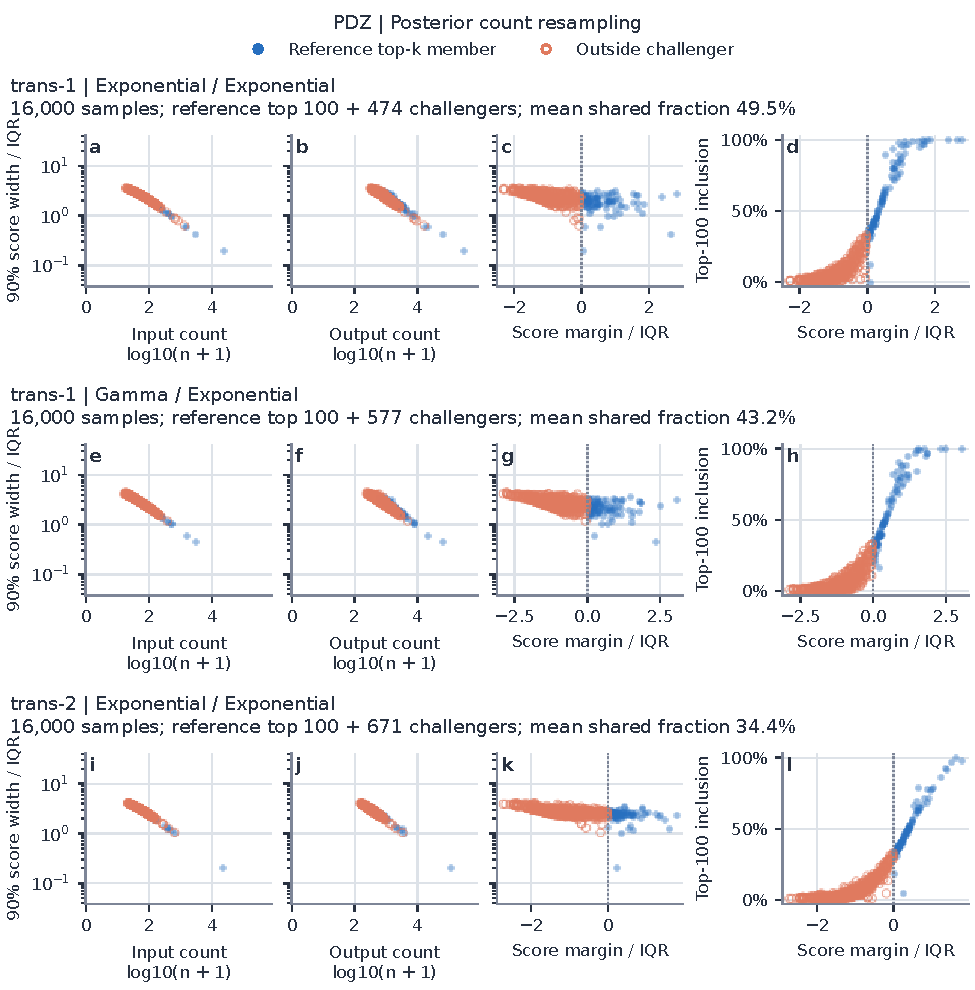
\includegraphics[width=\linewidth]{summary_why_posterior_predictive_pdz_01.pdf}
\caption{PDZ decision-cohort summaries: posterior count resampling. Rows, top to bottom: pdz-trans-1, Exponential--Exponential; pdz-trans-1, Gamma--Exponential; pdz-trans-2, Exponential--Exponential. Columns show normalized central 90\% score width versus input count, output count, and median-score margin from the top-100 cutoff; then top-100 inclusion versus that margin. Widths and margins use the run's top-1,000 median-score interquartile range (IQR). Blue filled points are reference top-100 members; orange open points are outside candidates with inclusion probability at least 0.01. Count and score-width limits are shared within family and scheme; margin limits are shared within a row. Dotted lines mark the cutoff. No regression lines are fitted.}
\label{fig:why-posterior_predictive-pdz-1}
\end{figure}
\clearpage

\begin{figure}[p]
\centering
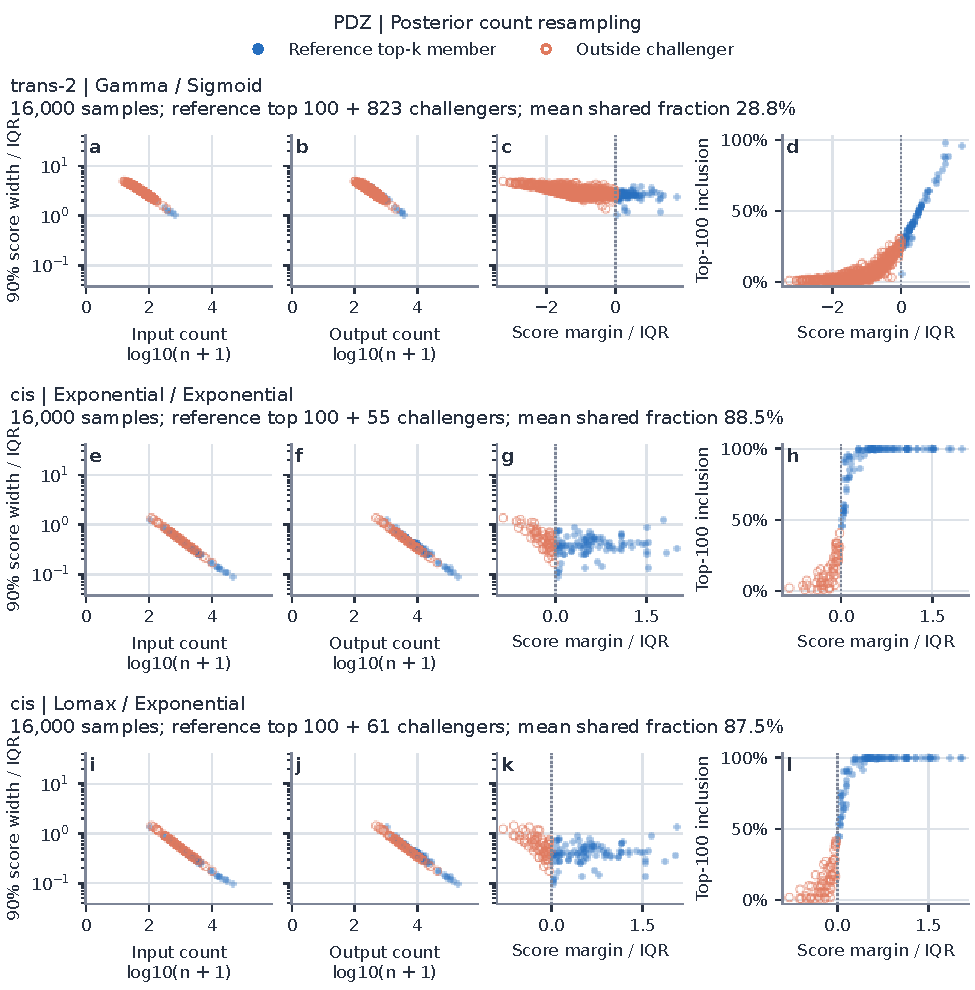
\includegraphics[width=\linewidth]{summary_why_posterior_predictive_pdz_02.pdf}
\caption{PDZ decision-cohort summaries: posterior count resampling. Rows, top to bottom: pdz-trans-2, Gamma--Sigmoid; pdz-cis, Exponential--Exponential; pdz-cis, Lomax--Exponential. Columns show normalized central 90\% score width versus input count, output count, and median-score margin from the top-100 cutoff; then top-100 inclusion versus that margin. Widths and margins use the run's top-1,000 median-score interquartile range (IQR). Blue filled points are reference top-100 members; orange open points are outside candidates with inclusion probability at least 0.01. Count and score-width limits are shared within family and scheme; margin limits are shared within a row. Dotted lines mark the cutoff. No regression lines are fitted.}
\label{fig:why-posterior_predictive-pdz-2}
\end{figure}
\clearpage

\begin{figure}[p]
\centering
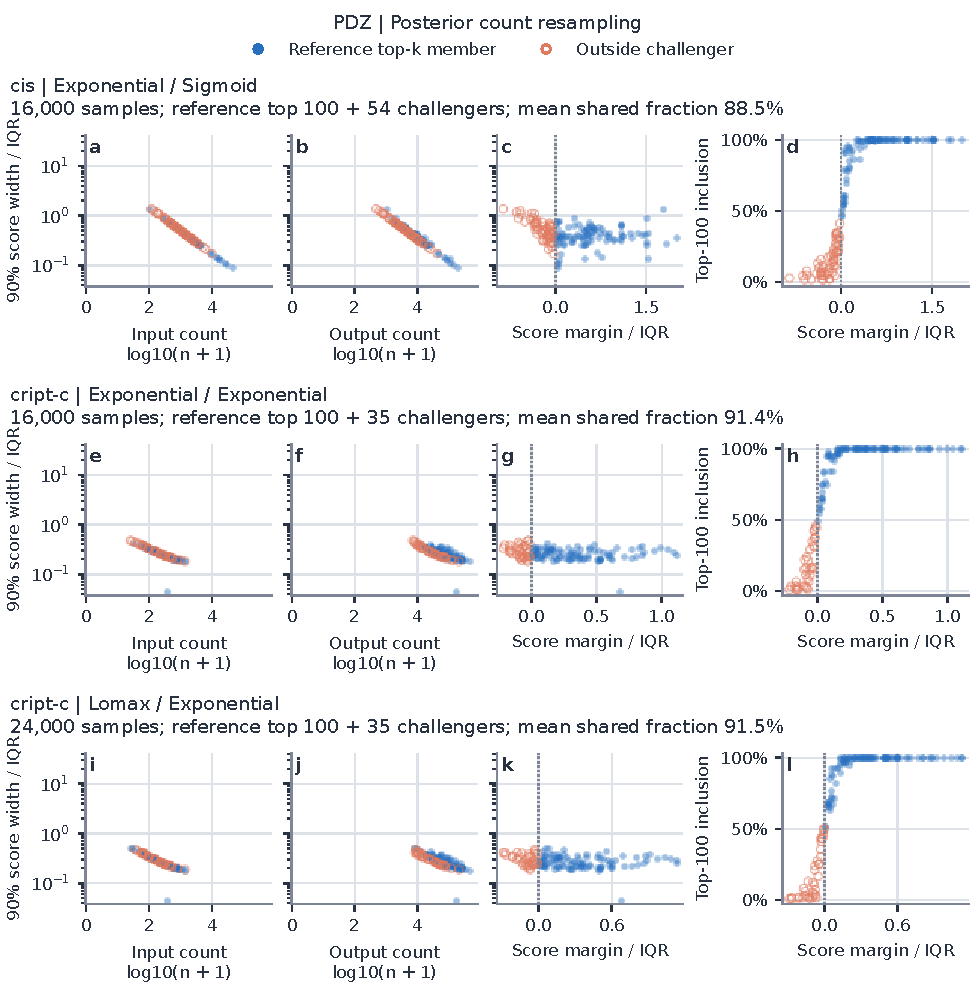
\includegraphics[width=\linewidth]{summary_why_posterior_predictive_pdz_03.pdf}
\caption{PDZ decision-cohort summaries: posterior count resampling. Rows, top to bottom: pdz-cis, Exponential--Sigmoid; pdz-cript-c, Exponential--Exponential; pdz-cript-c, Lomax--Exponential. Columns show normalized central 90\% score width versus input count, output count, and median-score margin from the top-100 cutoff; then top-100 inclusion versus that margin. Widths and margins use the run's top-1,000 median-score interquartile range (IQR). Blue filled points are reference top-100 members; orange open points are outside candidates with inclusion probability at least 0.01. Count and score-width limits are shared within family and scheme; margin limits are shared within a row. Dotted lines mark the cutoff. No regression lines are fitted.}
\label{fig:why-posterior_predictive-pdz-3}
\end{figure}
\clearpage

\begin{figure}[p]
\centering
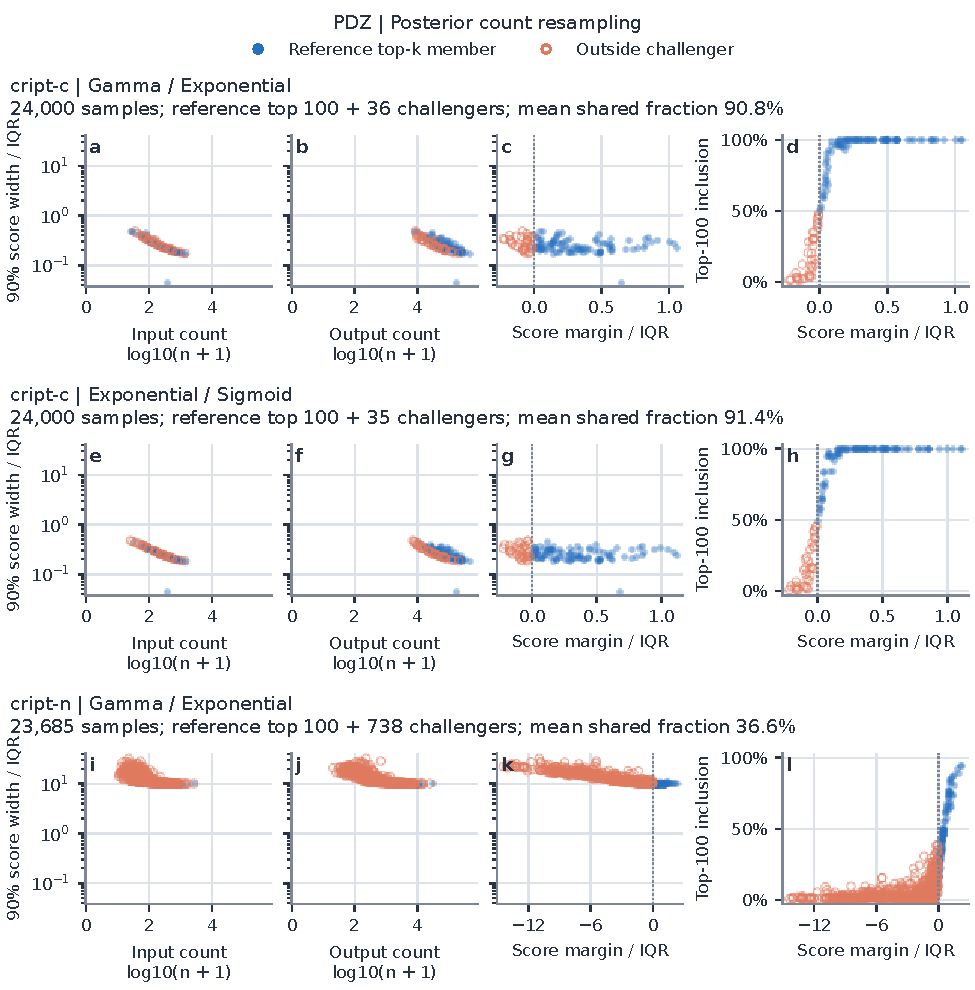
\includegraphics[width=\linewidth]{summary_why_posterior_predictive_pdz_04.pdf}
\caption{PDZ decision-cohort summaries: posterior count resampling. Rows, top to bottom: pdz-cript-c, Gamma--Exponential; pdz-cript-c, Exponential--Sigmoid; pdz-cript-n, Gamma--Exponential. Columns show normalized central 90\% score width versus input count, output count, and median-score margin from the top-100 cutoff; then top-100 inclusion versus that margin. Widths and margins use the run's top-1,000 median-score interquartile range (IQR). Blue filled points are reference top-100 members; orange open points are outside candidates with inclusion probability at least 0.01. Count and score-width limits are shared within family and scheme; margin limits are shared within a row. Dotted lines mark the cutoff. No regression lines are fitted.}
\label{fig:why-posterior_predictive-pdz-4}
\end{figure}
\clearpage

\begin{figure}[p]
\centering
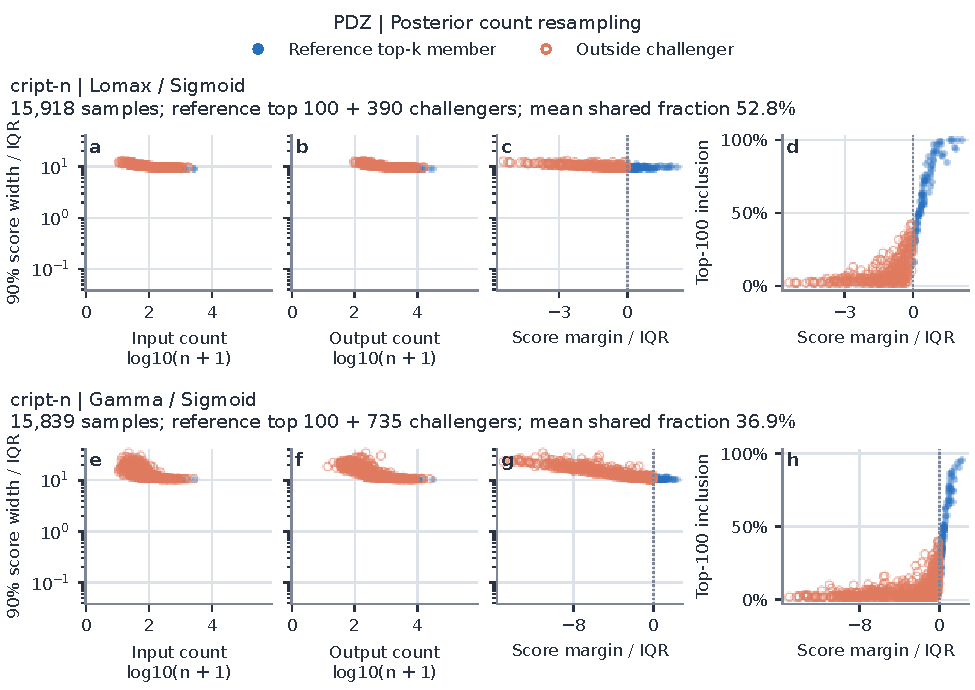
\includegraphics[width=\linewidth]{summary_why_posterior_predictive_pdz_05.pdf}
\caption{PDZ decision-cohort summaries: posterior count resampling. Rows, top to bottom: pdz-cript-n, Lomax--Sigmoid; pdz-cript-n, Gamma--Sigmoid. Columns show normalized central 90\% score width versus input count, output count, and median-score margin from the top-100 cutoff; then top-100 inclusion versus that margin. Widths and margins use the run's top-1,000 median-score interquartile range (IQR). Blue filled points are reference top-100 members; orange open points are outside candidates with inclusion probability at least 0.01. Count and score-width limits are shared within family and scheme; margin limits are shared within a row. Dotted lines mark the cutoff. No regression lines are fitted.}
\label{fig:why-posterior_predictive-pdz-5}
\end{figure}
\clearpage

\begin{figure}[p]
\centering
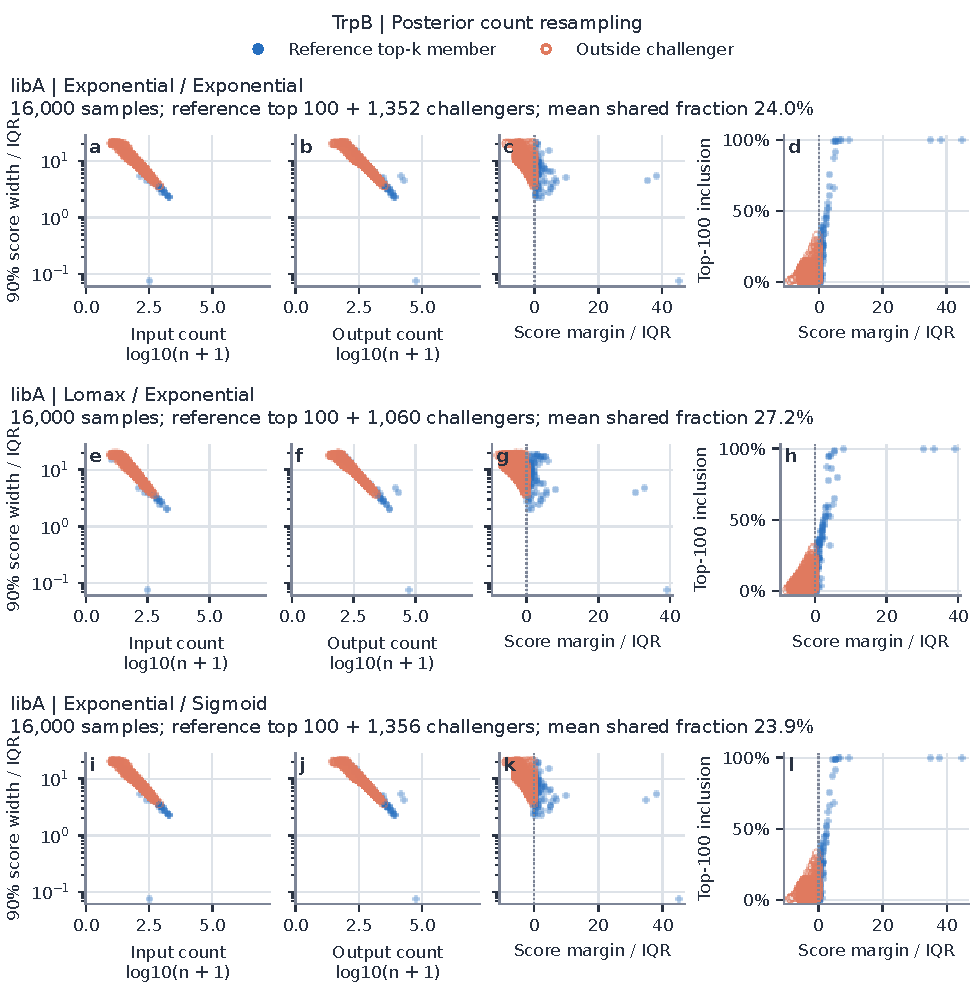
\includegraphics[width=\linewidth]{summary_why_posterior_predictive_trpb_01.pdf}
\caption{TrpB decision-cohort summaries: posterior count resampling. Rows, top to bottom: trpb-libA, Exponential--Exponential; trpb-libA, Lomax--Exponential; trpb-libA, Exponential--Sigmoid. Columns show normalized central 90\% score width versus input count, output count, and median-score margin from the top-100 cutoff; then top-100 inclusion versus that margin. Widths and margins use the run's top-1,000 median-score interquartile range (IQR). Blue filled points are reference top-100 members; orange open points are outside candidates with inclusion probability at least 0.01. Count and score-width limits are shared within family and scheme; margin limits are shared within a row. Dotted lines mark the cutoff. No regression lines are fitted.}
\label{fig:why-posterior_predictive-trpb-1}
\end{figure}
\clearpage

\begin{figure}[p]
\centering
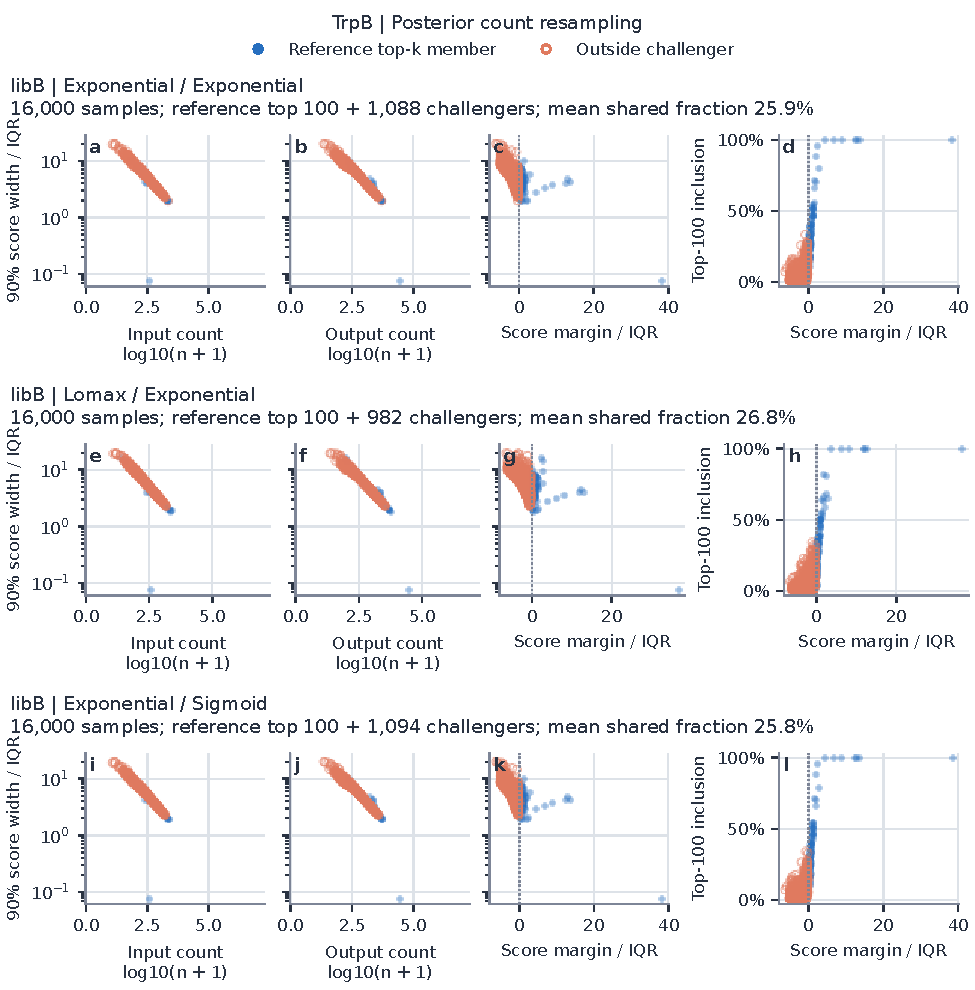
\includegraphics[width=\linewidth]{summary_why_posterior_predictive_trpb_02.pdf}
\caption{TrpB decision-cohort summaries: posterior count resampling. Rows, top to bottom: trpb-libB, Exponential--Exponential; trpb-libB, Lomax--Exponential; trpb-libB, Exponential--Sigmoid. Columns show normalized central 90\% score width versus input count, output count, and median-score margin from the top-100 cutoff; then top-100 inclusion versus that margin. Widths and margins use the run's top-1,000 median-score interquartile range (IQR). Blue filled points are reference top-100 members; orange open points are outside candidates with inclusion probability at least 0.01. Count and score-width limits are shared within family and scheme; margin limits are shared within a row. Dotted lines mark the cutoff. No regression lines are fitted.}
\label{fig:why-posterior_predictive-trpb-2}
\end{figure}
\clearpage

\begin{figure}[p]
\centering
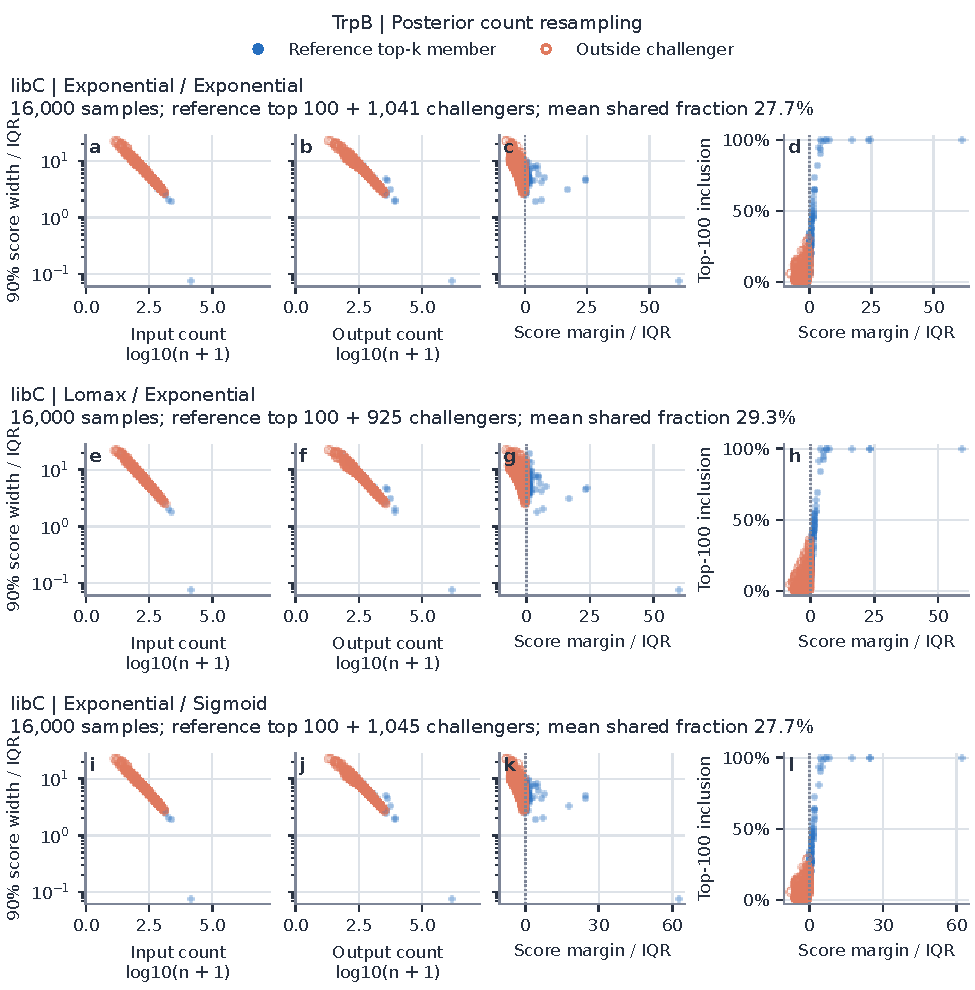
\includegraphics[width=\linewidth]{summary_why_posterior_predictive_trpb_03.pdf}
\caption{TrpB decision-cohort summaries: posterior count resampling. Rows, top to bottom: trpb-libC, Exponential--Exponential; trpb-libC, Lomax--Exponential; trpb-libC, Exponential--Sigmoid. Columns show normalized central 90\% score width versus input count, output count, and median-score margin from the top-100 cutoff; then top-100 inclusion versus that margin. Widths and margins use the run's top-1,000 median-score interquartile range (IQR). Blue filled points are reference top-100 members; orange open points are outside candidates with inclusion probability at least 0.01. Count and score-width limits are shared within family and scheme; margin limits are shared within a row. Dotted lines mark the cutoff. No regression lines are fitted.}
\label{fig:why-posterior_predictive-trpb-3}
\end{figure}
\clearpage

\begin{figure}[p]
\centering
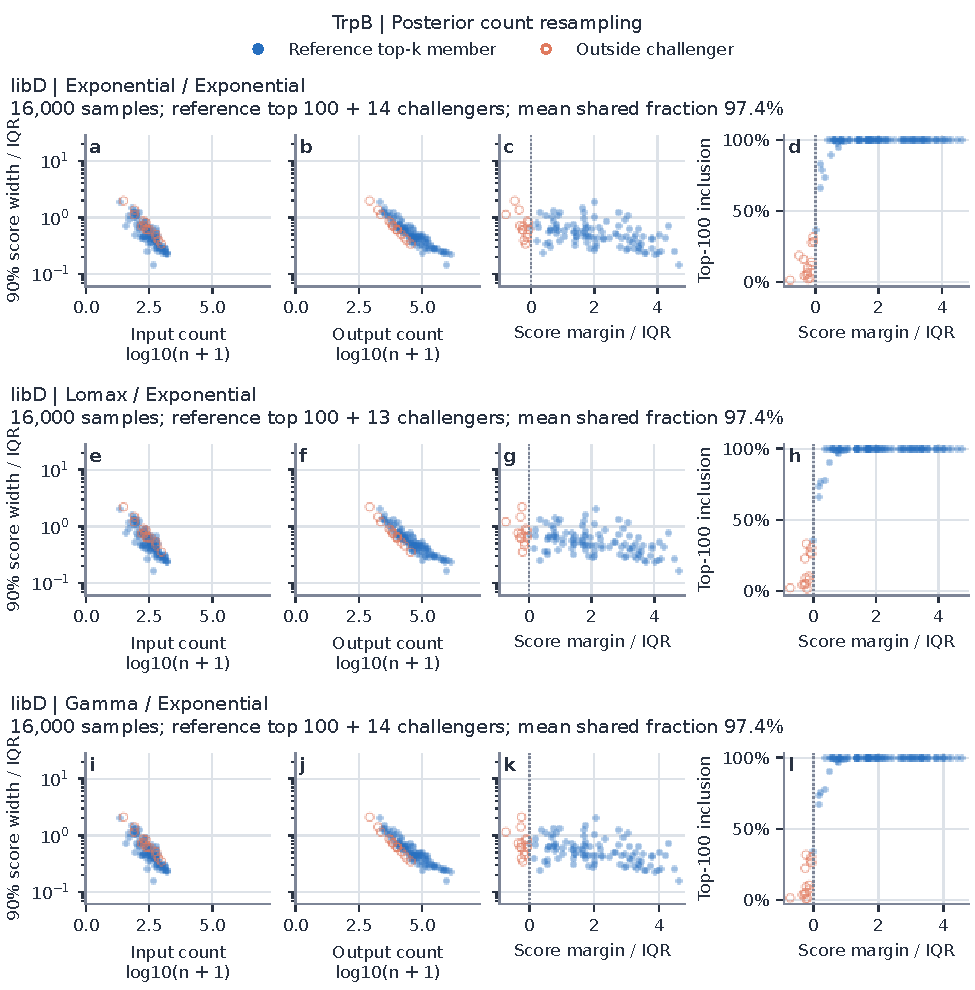
\includegraphics[width=\linewidth]{summary_why_posterior_predictive_trpb_04.pdf}
\caption{TrpB decision-cohort summaries: posterior count resampling. Rows, top to bottom: trpb-libD, Exponential--Exponential; trpb-libD, Lomax--Exponential; trpb-libD, Gamma--Exponential. Columns show normalized central 90\% score width versus input count, output count, and median-score margin from the top-100 cutoff; then top-100 inclusion versus that margin. Widths and margins use the run's top-1,000 median-score interquartile range (IQR). Blue filled points are reference top-100 members; orange open points are outside candidates with inclusion probability at least 0.01. Count and score-width limits are shared within family and scheme; margin limits are shared within a row. Dotted lines mark the cutoff. No regression lines are fitted.}
\label{fig:why-posterior_predictive-trpb-4}
\end{figure}
\clearpage

\begin{figure}[p]
\centering
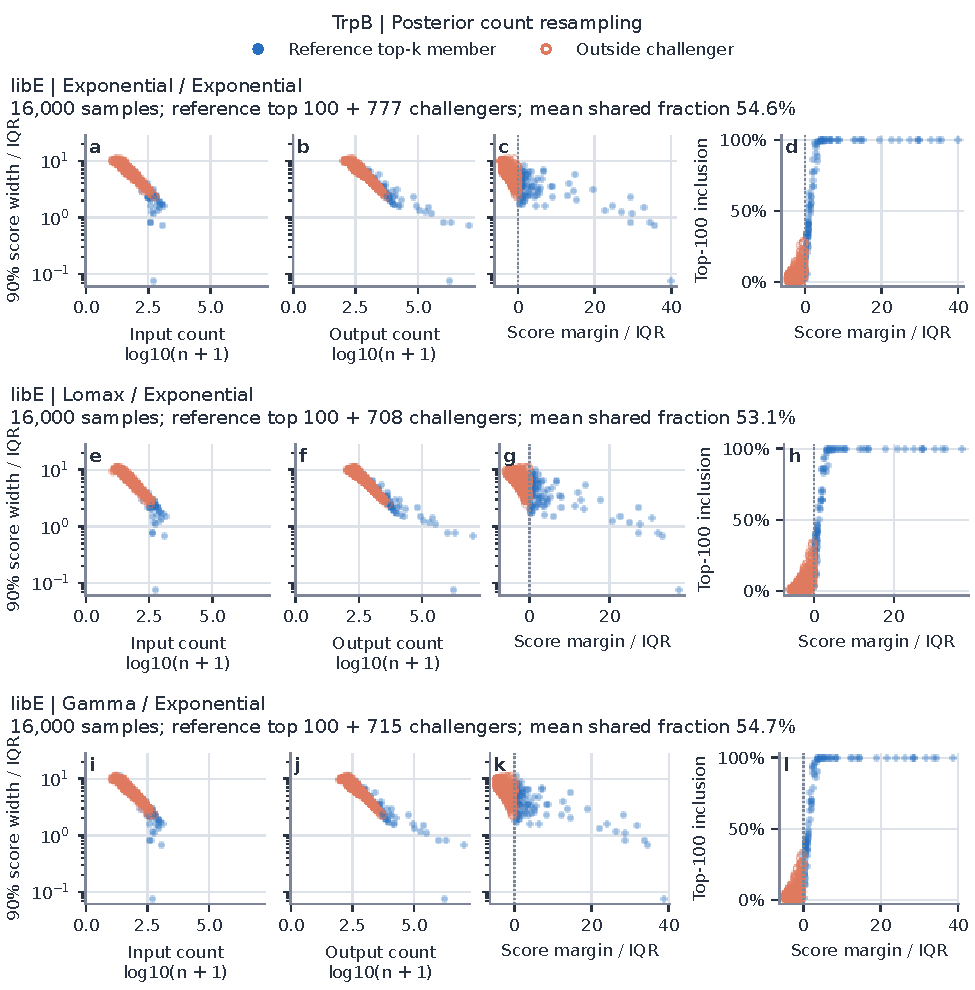
\includegraphics[width=\linewidth]{summary_why_posterior_predictive_trpb_05.pdf}
\caption{TrpB decision-cohort summaries: posterior count resampling. Rows, top to bottom: trpb-libE, Exponential--Exponential; trpb-libE, Lomax--Exponential; trpb-libE, Gamma--Exponential. Columns show normalized central 90\% score width versus input count, output count, and median-score margin from the top-100 cutoff; then top-100 inclusion versus that margin. Widths and margins use the run's top-1,000 median-score interquartile range (IQR). Blue filled points are reference top-100 members; orange open points are outside candidates with inclusion probability at least 0.01. Count and score-width limits are shared within family and scheme; margin limits are shared within a row. Dotted lines mark the cutoff. No regression lines are fitted.}
\label{fig:why-posterior_predictive-trpb-5}
\end{figure}
\clearpage

\begin{figure}[p]
\centering
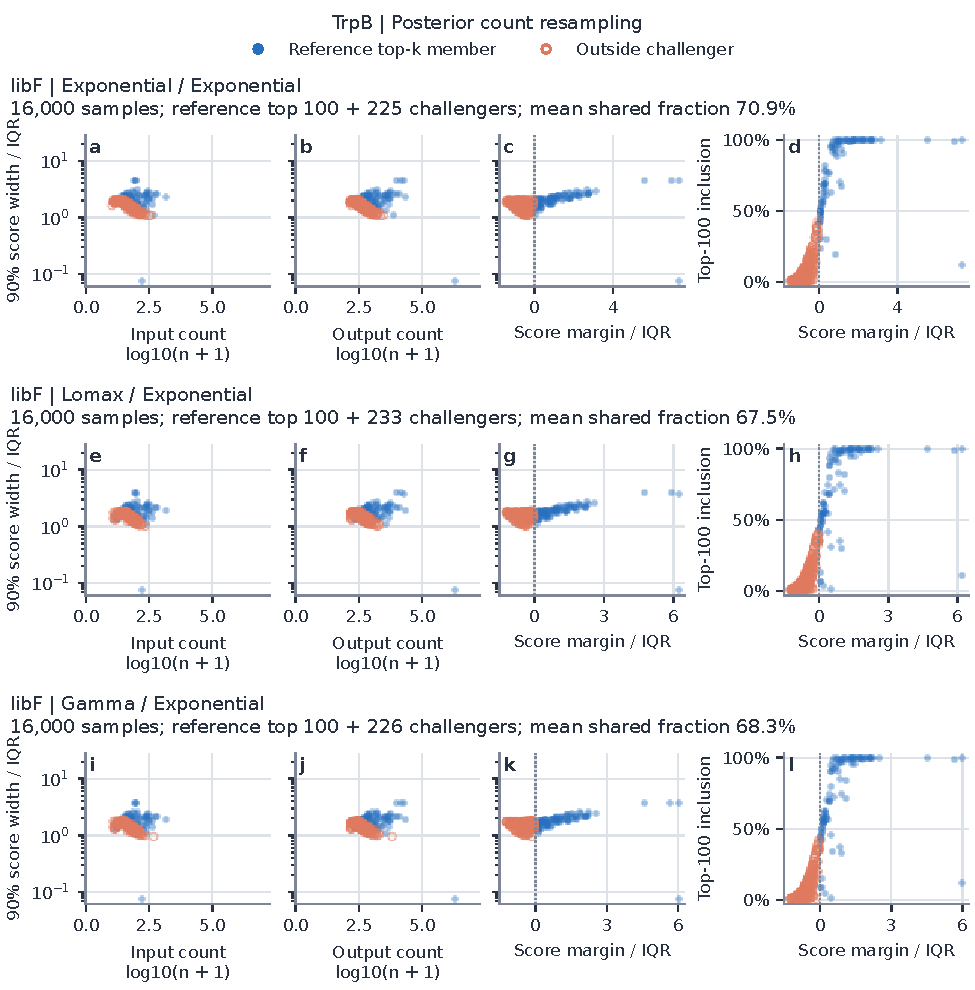
\includegraphics[width=\linewidth]{summary_why_posterior_predictive_trpb_06.pdf}
\caption{TrpB decision-cohort summaries: posterior count resampling. Rows, top to bottom: trpb-libF, Exponential--Exponential; trpb-libF, Lomax--Exponential; trpb-libF, Gamma--Exponential. Columns show normalized central 90\% score width versus input count, output count, and median-score margin from the top-100 cutoff; then top-100 inclusion versus that margin. Widths and margins use the run's top-1,000 median-score interquartile range (IQR). Blue filled points are reference top-100 members; orange open points are outside candidates with inclusion probability at least 0.01. Count and score-width limits are shared within family and scheme; margin limits are shared within a row. Dotted lines mark the cutoff. No regression lines are fitted.}
\label{fig:why-posterior_predictive-trpb-6}
\end{figure}
\clearpage

\begin{figure}[p]
\centering
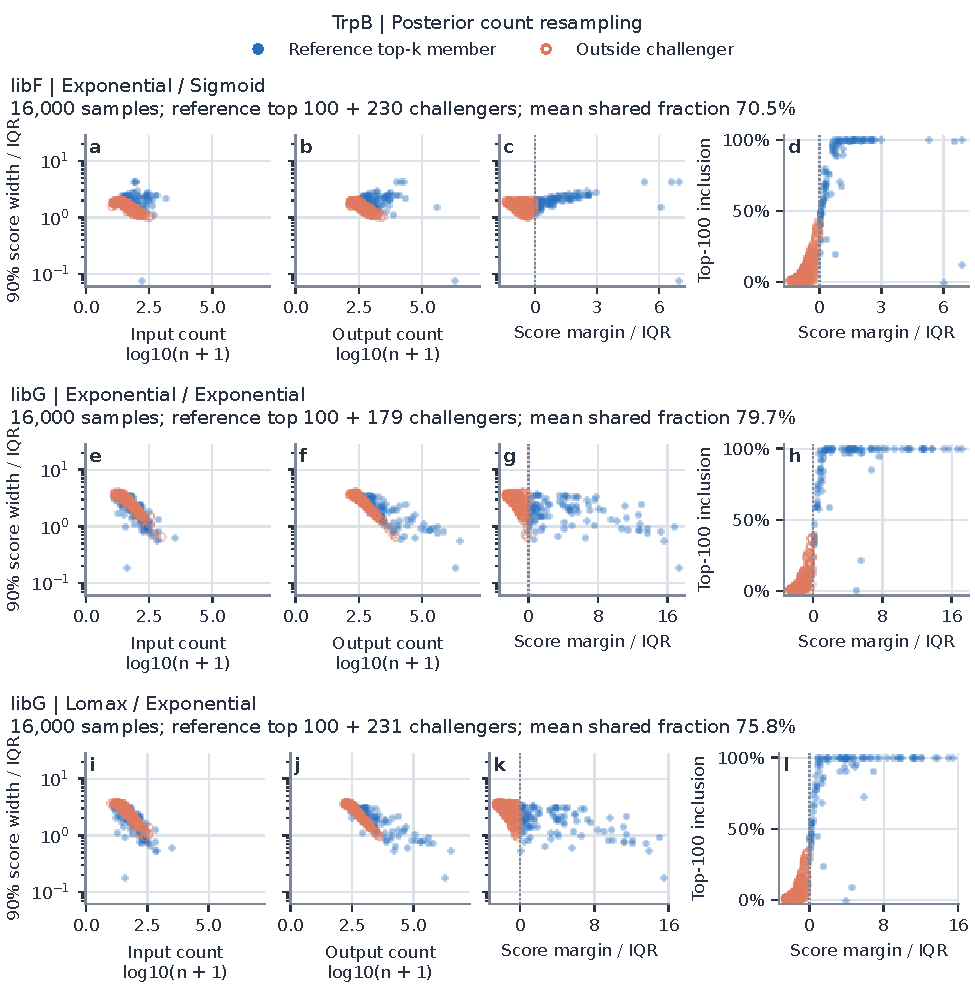
\includegraphics[width=\linewidth]{summary_why_posterior_predictive_trpb_07.pdf}
\caption{TrpB decision-cohort summaries: posterior count resampling. Rows, top to bottom: trpb-libF, Exponential--Sigmoid; trpb-libG, Exponential--Exponential; trpb-libG, Lomax--Exponential. Columns show normalized central 90\% score width versus input count, output count, and median-score margin from the top-100 cutoff; then top-100 inclusion versus that margin. Widths and margins use the run's top-1,000 median-score interquartile range (IQR). Blue filled points are reference top-100 members; orange open points are outside candidates with inclusion probability at least 0.01. Count and score-width limits are shared within family and scheme; margin limits are shared within a row. Dotted lines mark the cutoff. No regression lines are fitted.}
\label{fig:why-posterior_predictive-trpb-7}
\end{figure}
\clearpage

\begin{figure}[p]
\centering
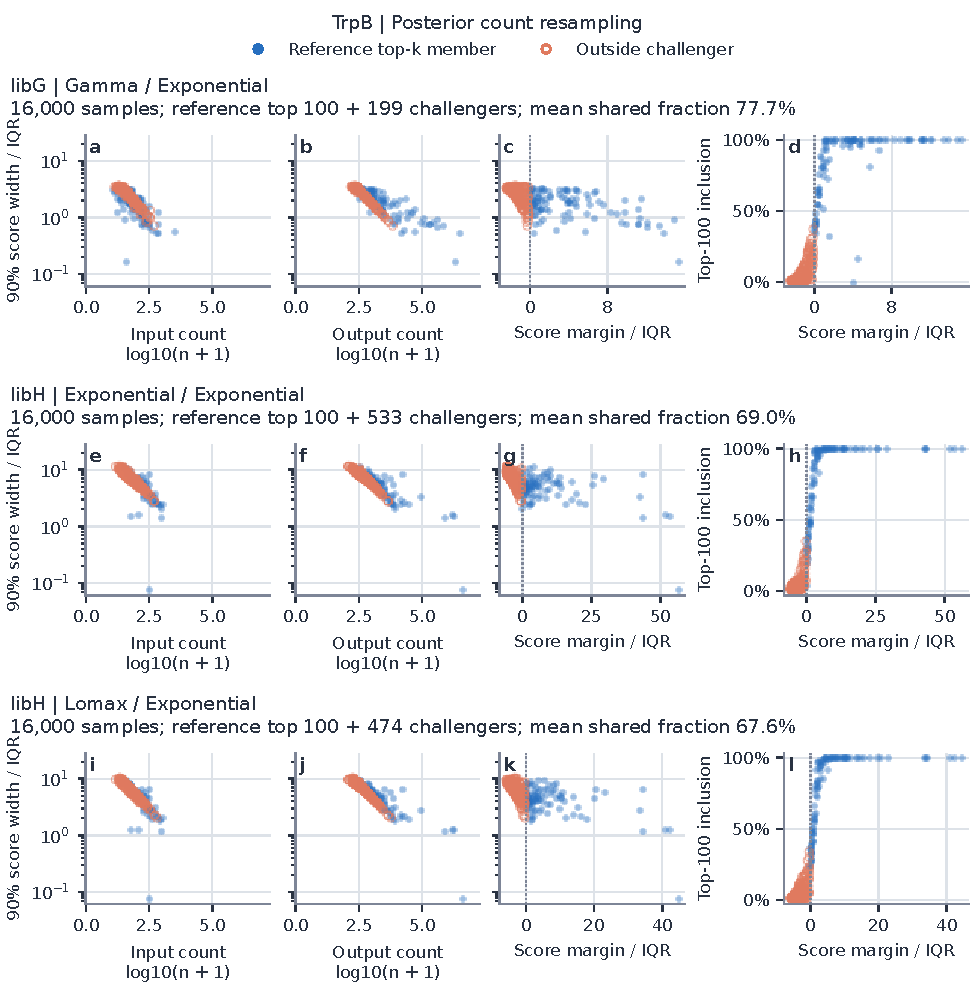
\includegraphics[width=\linewidth]{summary_why_posterior_predictive_trpb_08.pdf}
\caption{TrpB decision-cohort summaries: posterior count resampling. Rows, top to bottom: trpb-libG, Gamma--Exponential; trpb-libH, Exponential--Exponential; trpb-libH, Lomax--Exponential. Columns show normalized central 90\% score width versus input count, output count, and median-score margin from the top-100 cutoff; then top-100 inclusion versus that margin. Widths and margins use the run's top-1,000 median-score interquartile range (IQR). Blue filled points are reference top-100 members; orange open points are outside candidates with inclusion probability at least 0.01. Count and score-width limits are shared within family and scheme; margin limits are shared within a row. Dotted lines mark the cutoff. No regression lines are fitted.}
\label{fig:why-posterior_predictive-trpb-8}
\end{figure}
\clearpage

\begin{figure}[p]
\centering
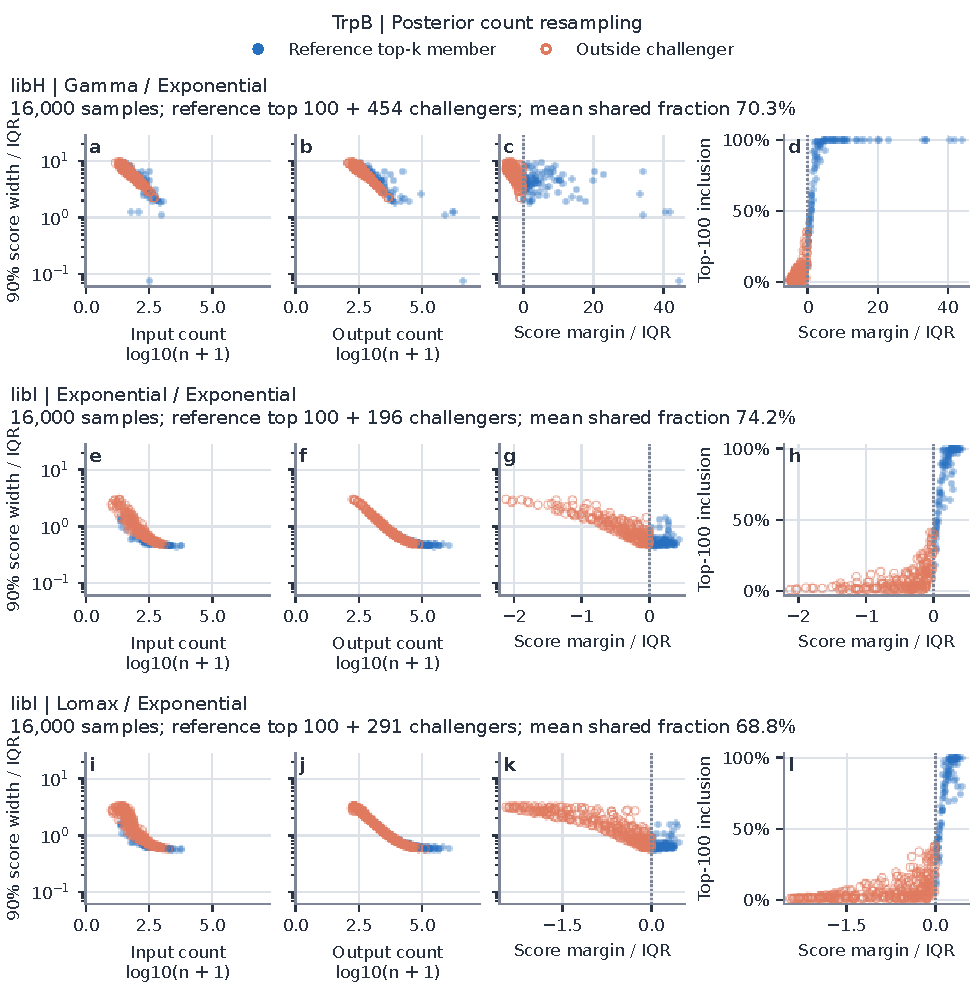
\includegraphics[width=\linewidth]{summary_why_posterior_predictive_trpb_09.pdf}
\caption{TrpB decision-cohort summaries: posterior count resampling. Rows, top to bottom: trpb-libH, Gamma--Exponential; trpb-libI, Exponential--Exponential; trpb-libI, Lomax--Exponential. Columns show normalized central 90\% score width versus input count, output count, and median-score margin from the top-100 cutoff; then top-100 inclusion versus that margin. Widths and margins use the run's top-1,000 median-score interquartile range (IQR). Blue filled points are reference top-100 members; orange open points are outside candidates with inclusion probability at least 0.01. Count and score-width limits are shared within family and scheme; margin limits are shared within a row. Dotted lines mark the cutoff. No regression lines are fitted.}
\label{fig:why-posterior_predictive-trpb-9}
\end{figure}
\clearpage

\begin{figure}[p]
\centering
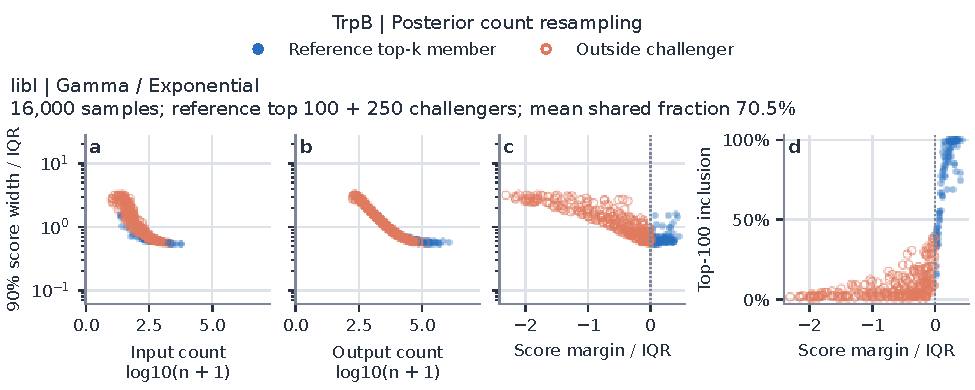
\includegraphics[width=\linewidth]{summary_why_posterior_predictive_trpb_10.pdf}
\caption{TrpB decision-cohort summaries: posterior count resampling. Rows, top to bottom: trpb-libI, Gamma--Exponential. Columns show normalized central 90\% score width versus input count, output count, and median-score margin from the top-100 cutoff; then top-100 inclusion versus that margin. Widths and margins use the run's top-1,000 median-score interquartile range (IQR). Blue filled points are reference top-100 members; orange open points are outside candidates with inclusion probability at least 0.01. Count and score-width limits are shared within family and scheme; margin limits are shared within a row. Dotted lines mark the cutoff. No regression lines are fitted.}
\label{fig:why-posterior_predictive-trpb-10}
\end{figure}
\clearpage

\begin{figure}[p]
\centering
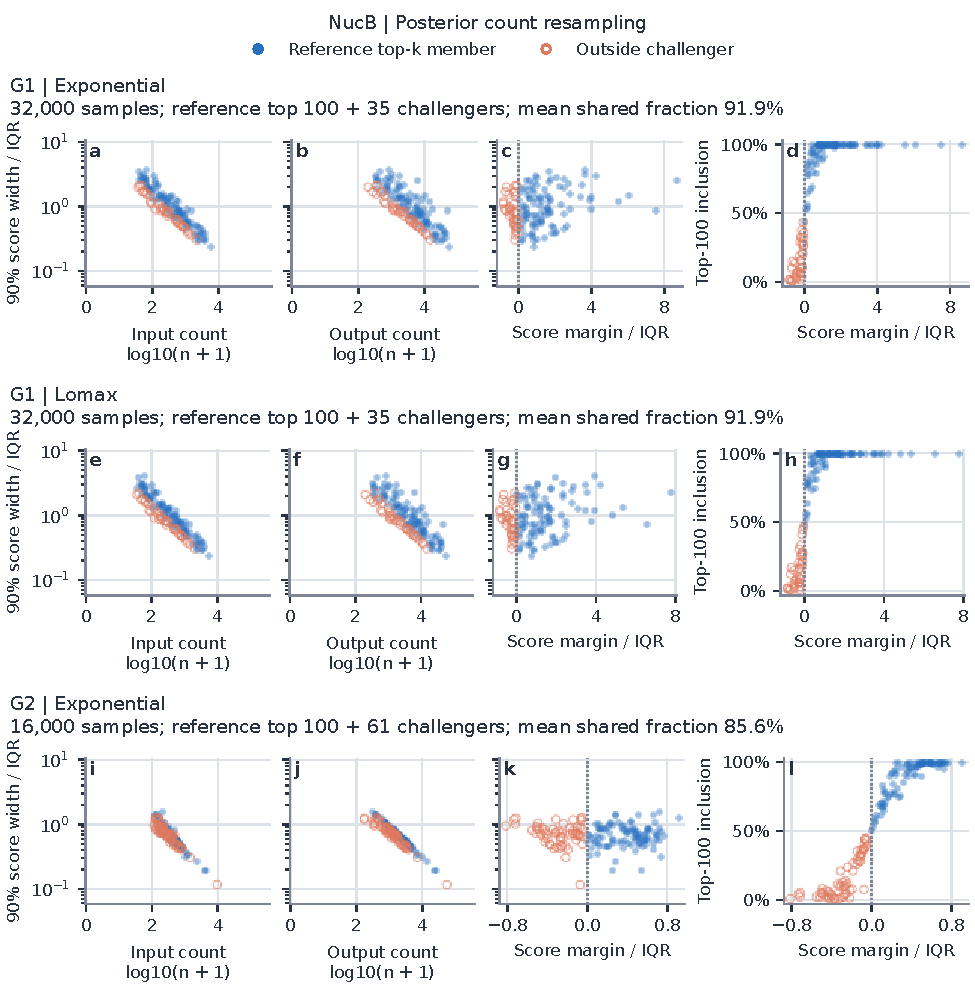
\includegraphics[width=\linewidth]{summary_why_posterior_predictive_nuc_01.pdf}
\caption{NucB decision-cohort summaries: posterior count resampling. Rows, top to bottom: nuc-G1, Exponential; nuc-G1, Lomax; nuc-G2, Exponential. Columns show normalized central 90\% score width versus input count, output count, and median-score margin from the top-100 cutoff; then top-100 inclusion versus that margin. Widths and margins use the run's top-1,000 median-score interquartile range (IQR). Blue filled points are reference top-100 members; orange open points are outside candidates with inclusion probability at least 0.01. Count and score-width limits are shared within family and scheme; margin limits are shared within a row. Dotted lines mark the cutoff. No regression lines are fitted.}
\label{fig:why-posterior_predictive-nuc-1}
\end{figure}
\clearpage

\begin{figure}[p]
\centering
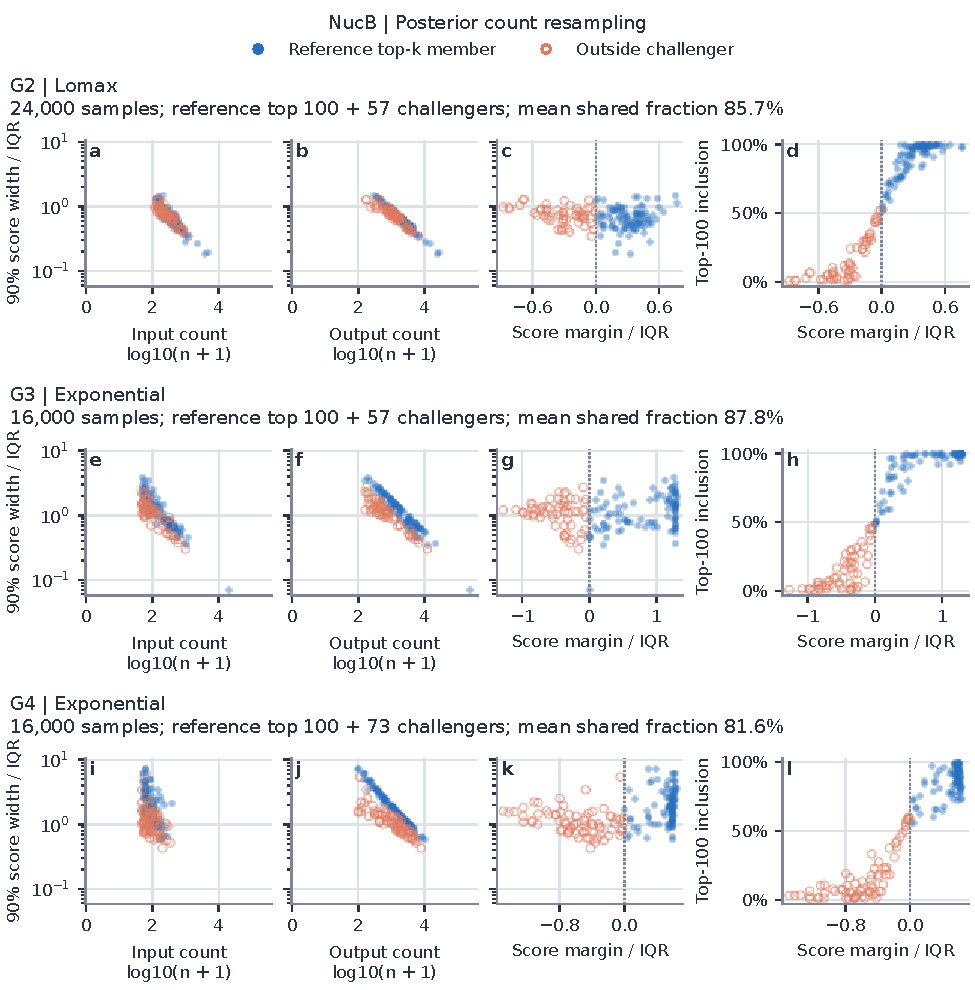
\includegraphics[width=\linewidth]{summary_why_posterior_predictive_nuc_02.pdf}
\caption{NucB decision-cohort summaries: posterior count resampling. Rows, top to bottom: nuc-G2, Lomax; nuc-G3, Exponential; nuc-G4, Exponential. Columns show normalized central 90\% score width versus input count, output count, and median-score margin from the top-100 cutoff; then top-100 inclusion versus that margin. Widths and margins use the run's top-1,000 median-score interquartile range (IQR). Blue filled points are reference top-100 members; orange open points are outside candidates with inclusion probability at least 0.01. Count and score-width limits are shared within family and scheme; margin limits are shared within a row. Dotted lines mark the cutoff. No regression lines are fitted.}
\label{fig:why-posterior_predictive-nuc-2}
\end{figure}
\clearpage

\begin{figure}[p]
\centering
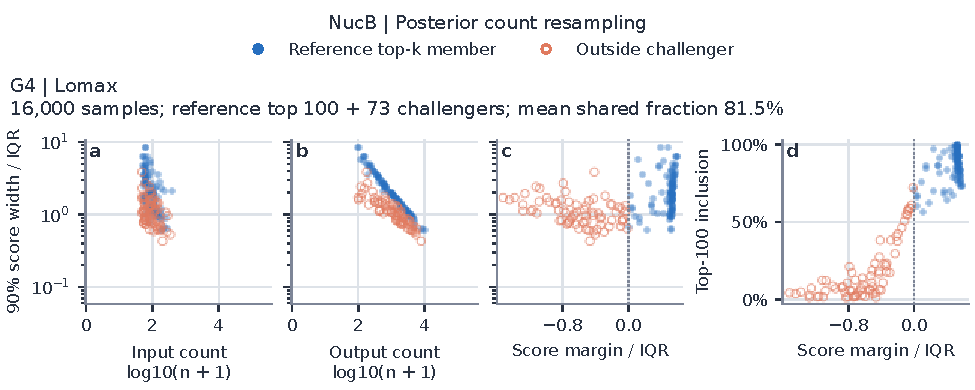
\includegraphics[width=\linewidth]{summary_why_posterior_predictive_nuc_03.pdf}
\caption{NucB decision-cohort summaries: posterior count resampling. Rows, top to bottom: nuc-G4, Lomax. Columns show normalized central 90\% score width versus input count, output count, and median-score margin from the top-100 cutoff; then top-100 inclusion versus that margin. Widths and margins use the run's top-1,000 median-score interquartile range (IQR). Blue filled points are reference top-100 members; orange open points are outside candidates with inclusion probability at least 0.01. Count and score-width limits are shared within family and scheme; margin limits are shared within a row. Dotted lines mark the cutoff. No regression lines are fitted.}
\label{fig:why-posterior_predictive-nuc-3}
\end{figure}
\clearpage
